\chapter[Results][Results]{Results}
\label{chap:results}

\begin{quote}
  Results of the $\Htautau$ analysis are described. This is described in additional detail in the recent ATLAS $\Htautau$ publication~\cite{HIGG-2013-32}. The description of the fit procedure draws heavily from the recent ATLAS $\HWW$ publication~\cite{HIGG-2013-13}.
\end{quote}

\section{Predictions in the signal region}
\label{sec:results-prefit}

\clearpage

\begin{figure}[tp]
  \centering
  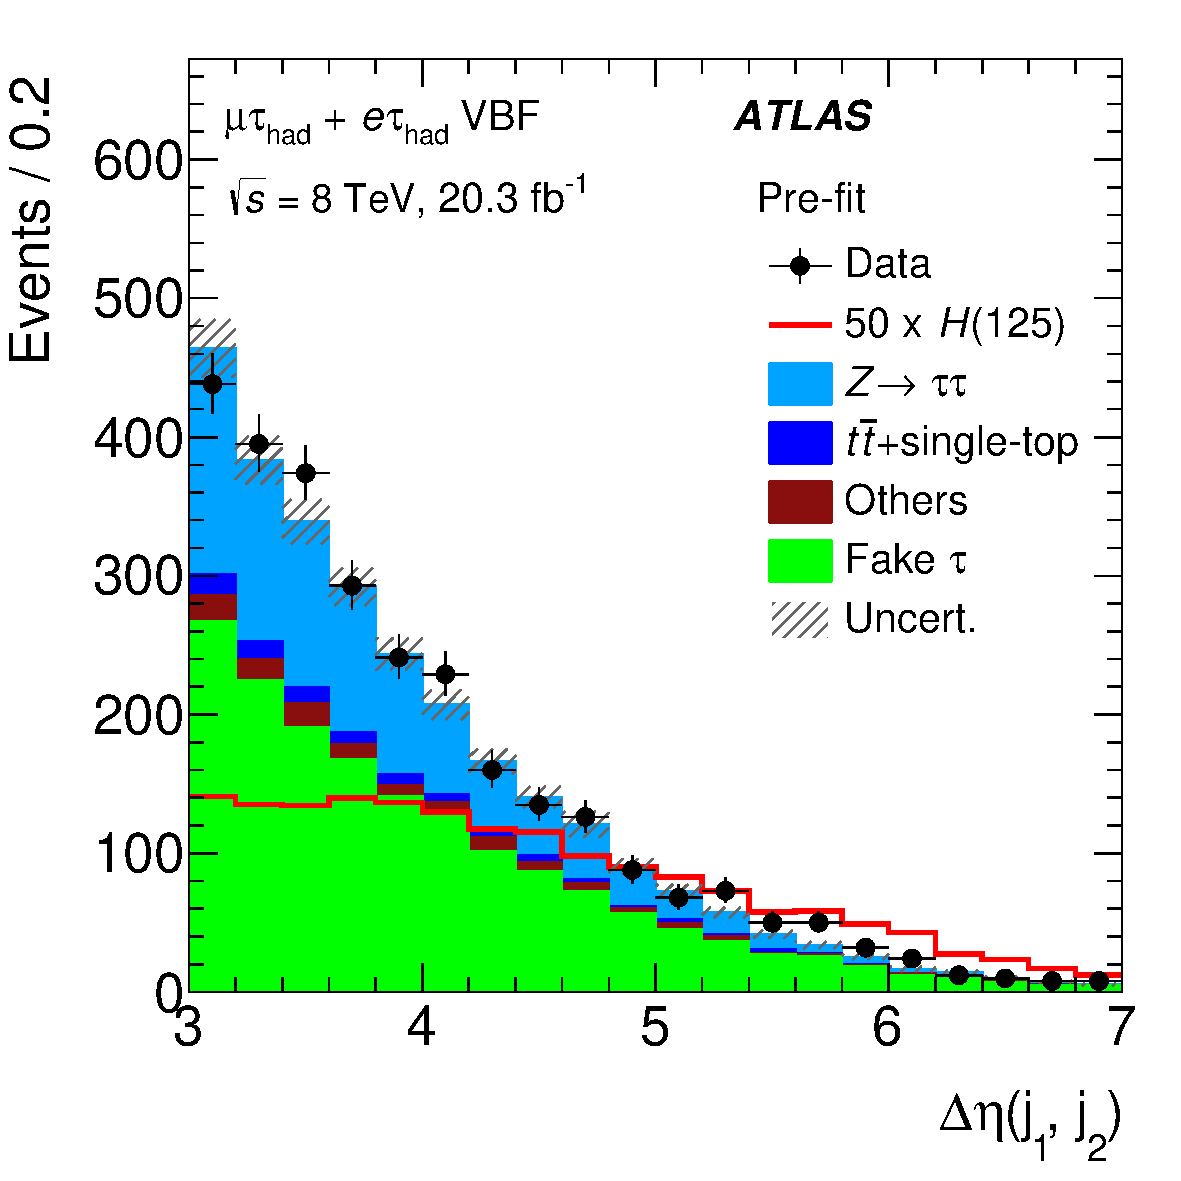
\includegraphics[width=0.30\textwidth]{figures/HIGG-2013-32/fig_02c}
  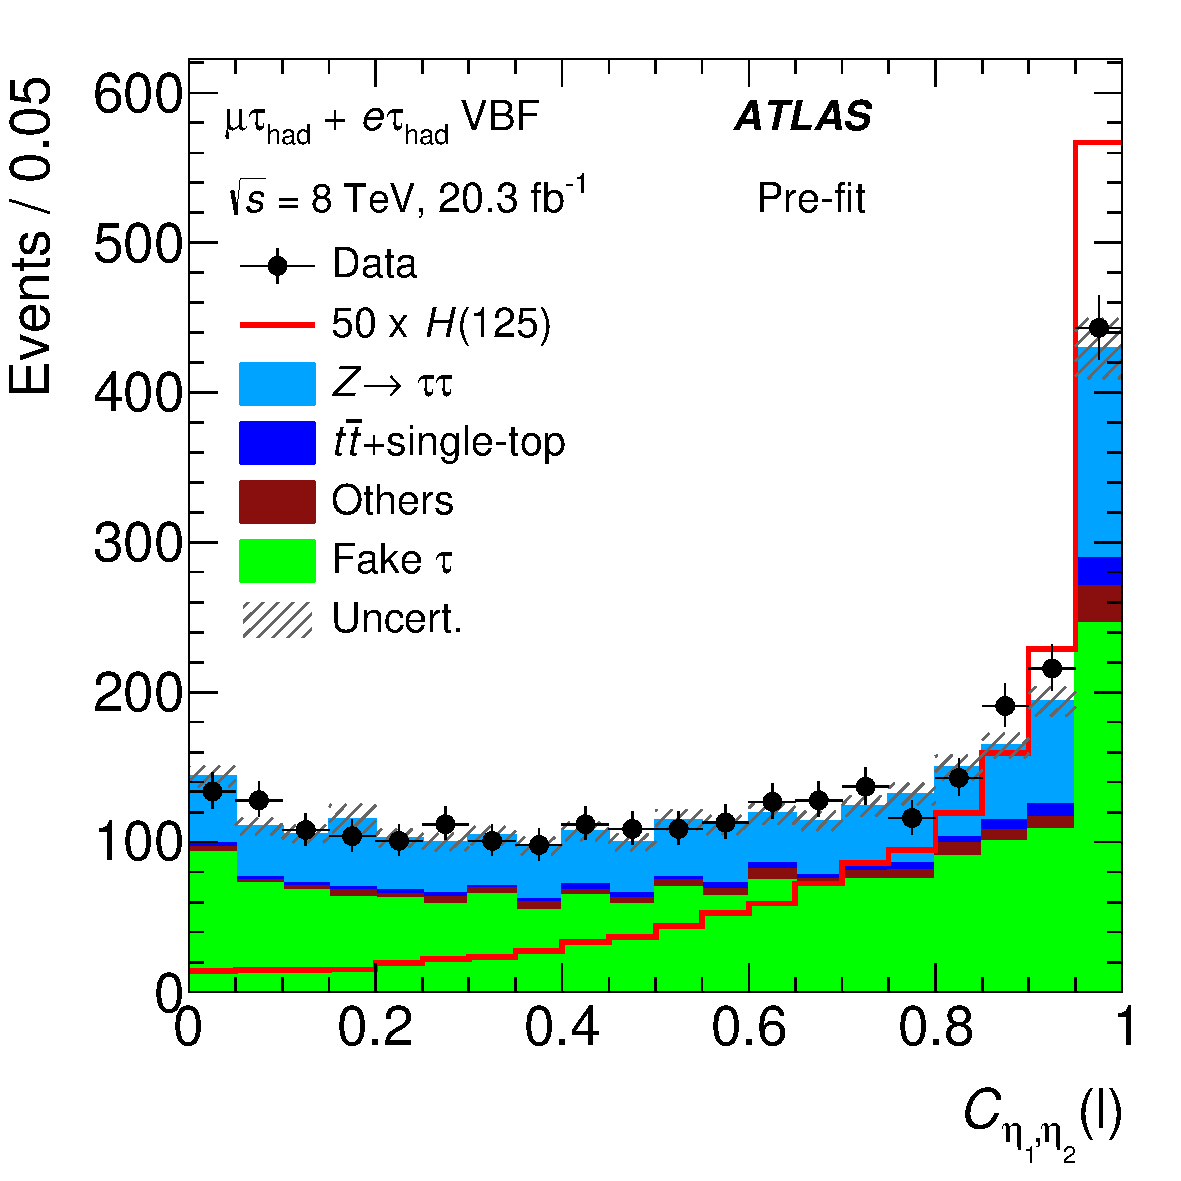
\includegraphics[width=0.30\textwidth]{figures/HIGG-2013-32/figaux_06a}
  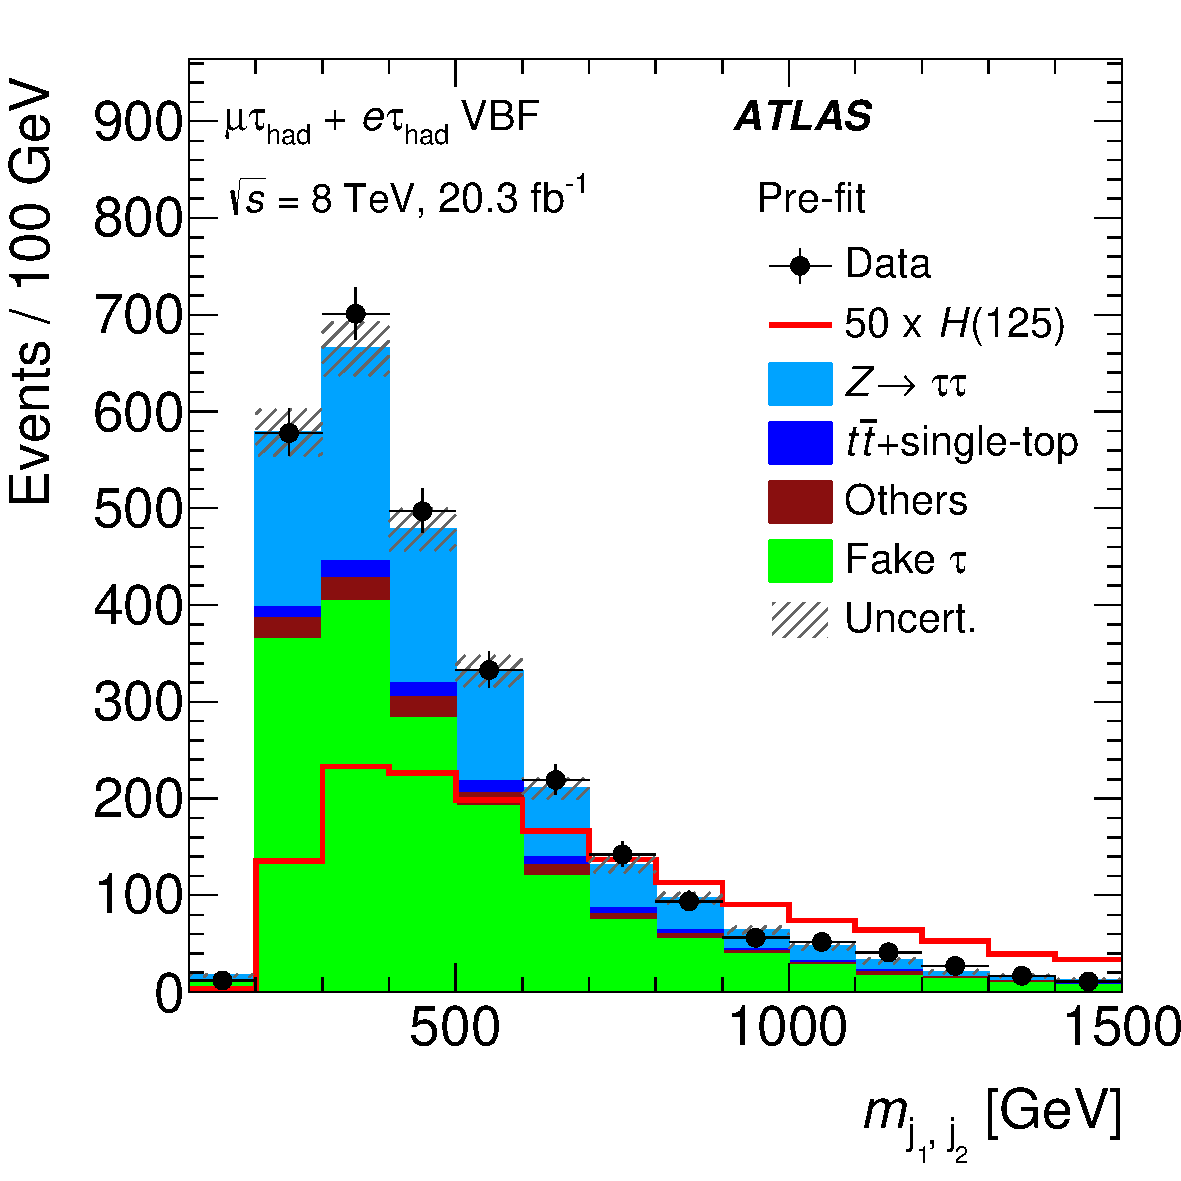
\includegraphics[width=0.30\textwidth]{figures/HIGG-2013-32/figaux_06b}
  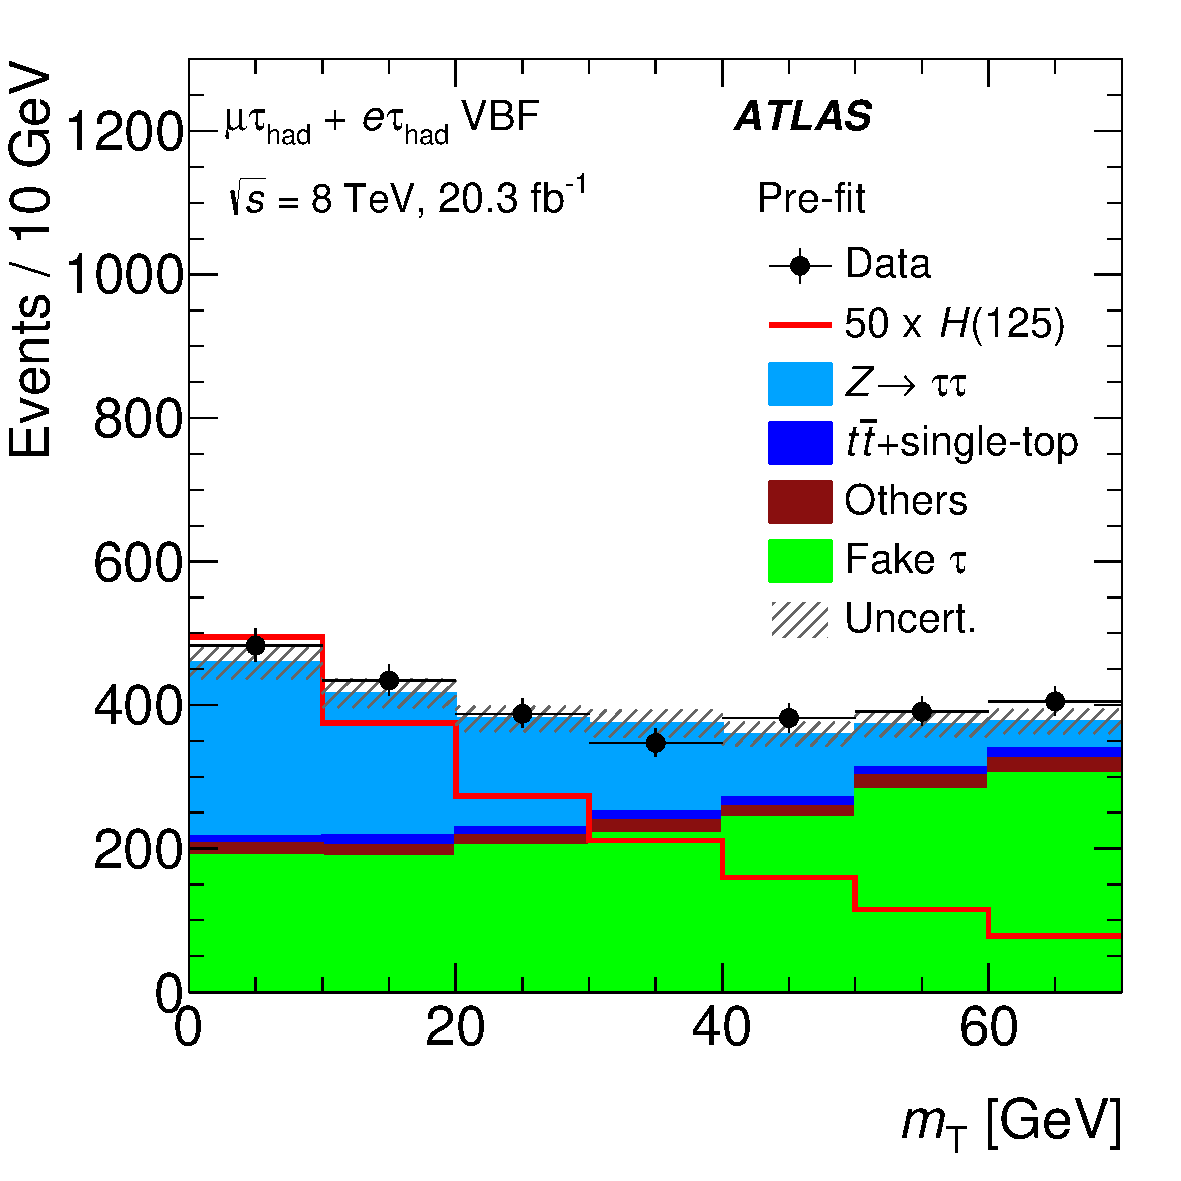
\includegraphics[width=0.30\textwidth]{figures/HIGG-2013-32/figaux_06c}
  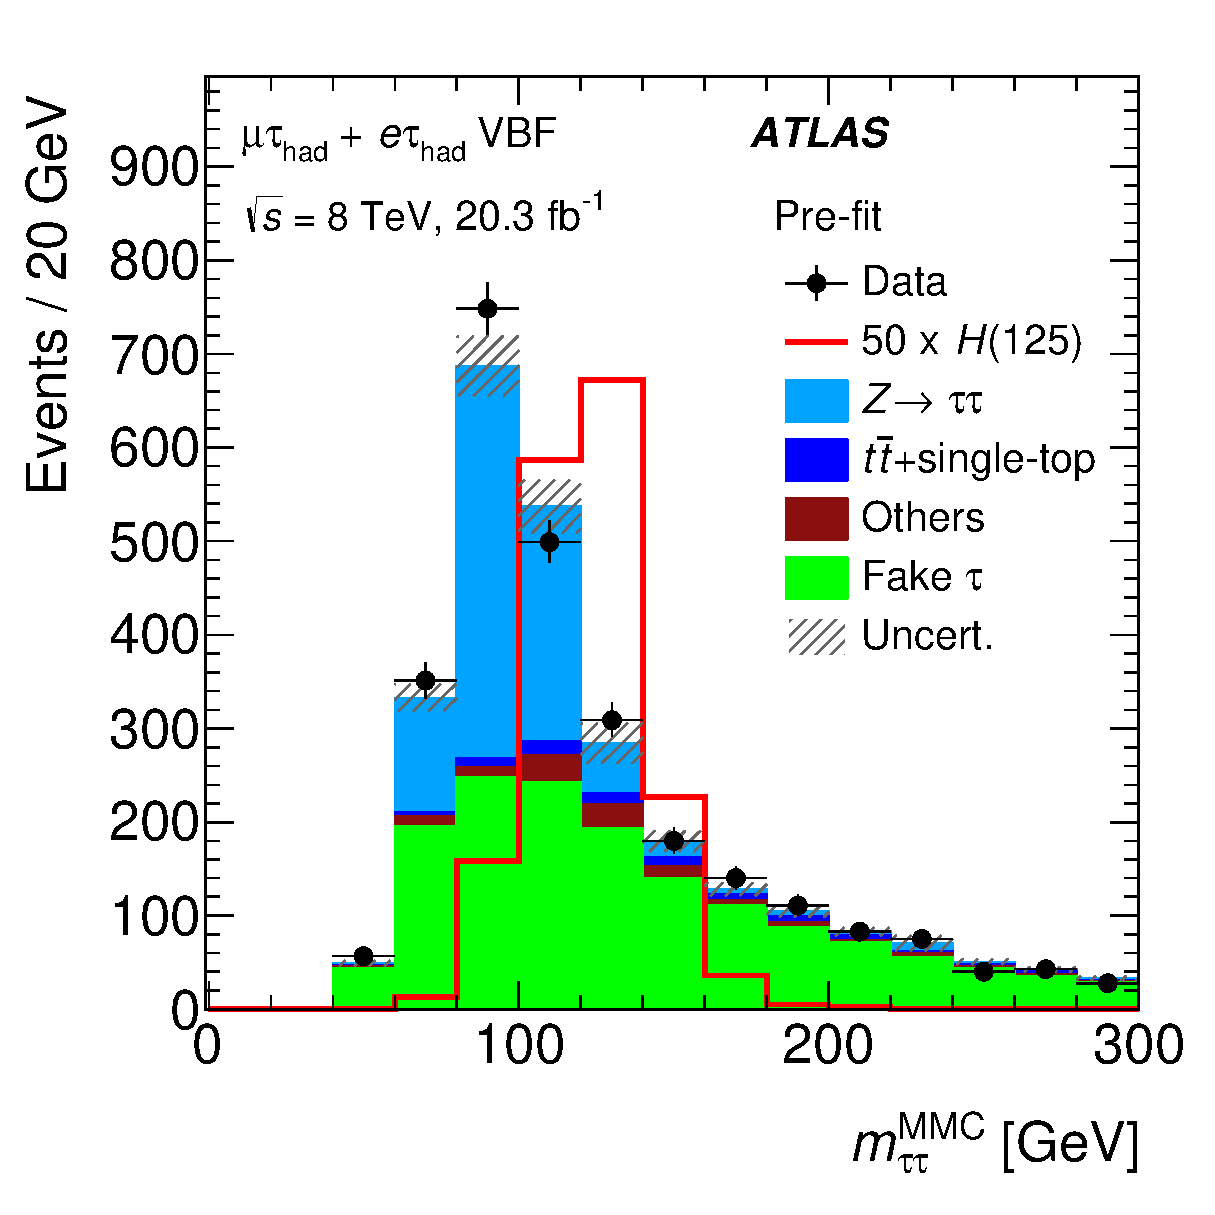
\includegraphics[width=0.30\textwidth]{figures/HIGG-2013-32/figaux_06d}
  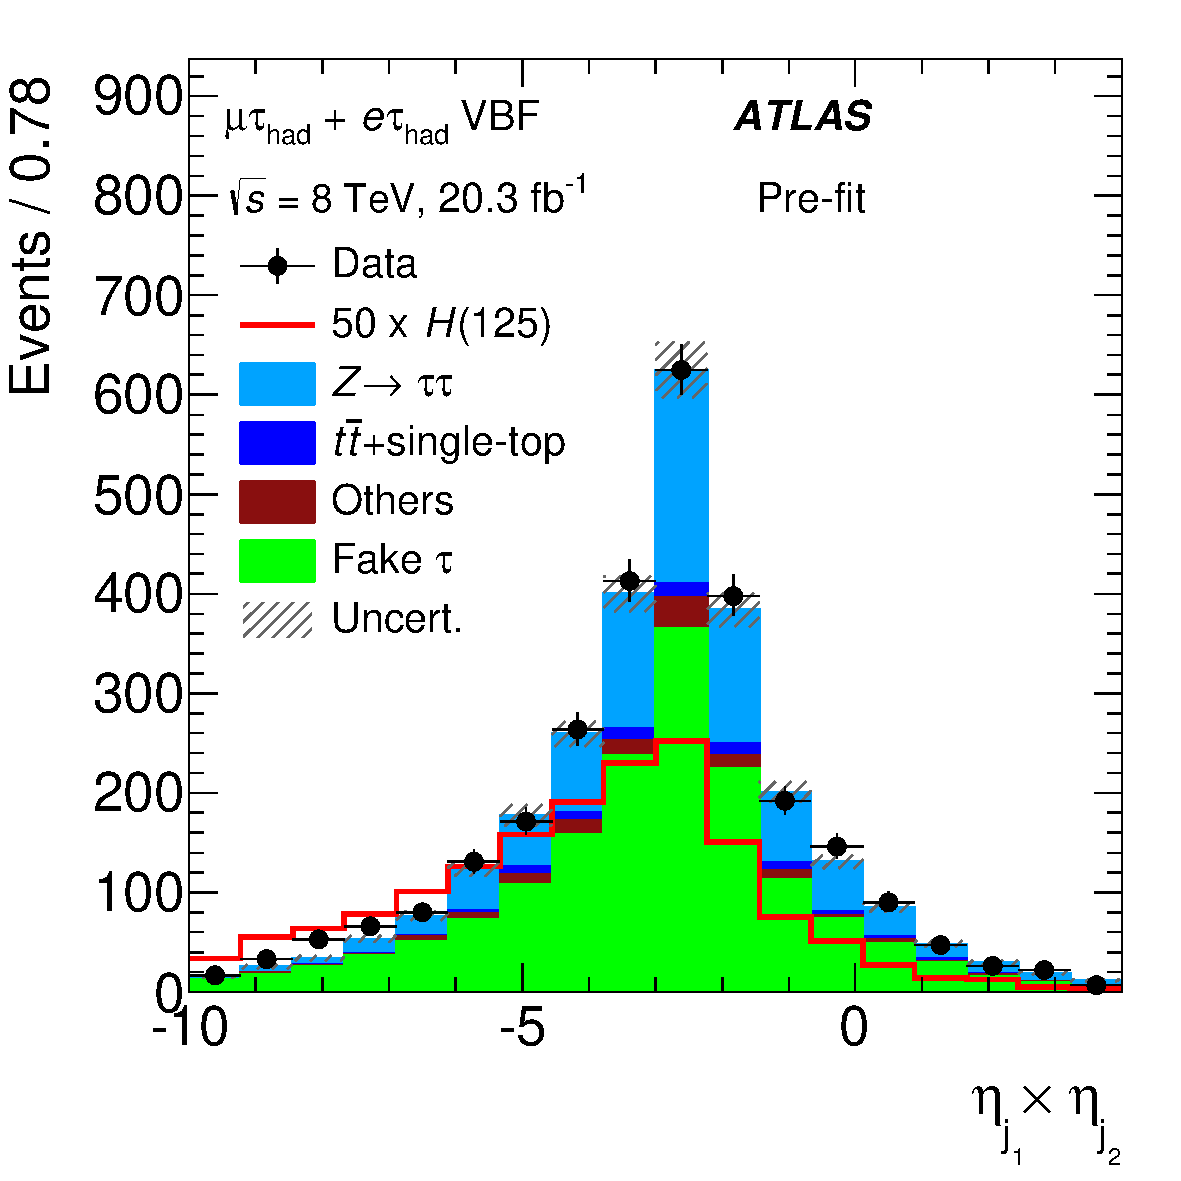
\includegraphics[width=0.30\textwidth]{figures/HIGG-2013-32/figaux_06e}
  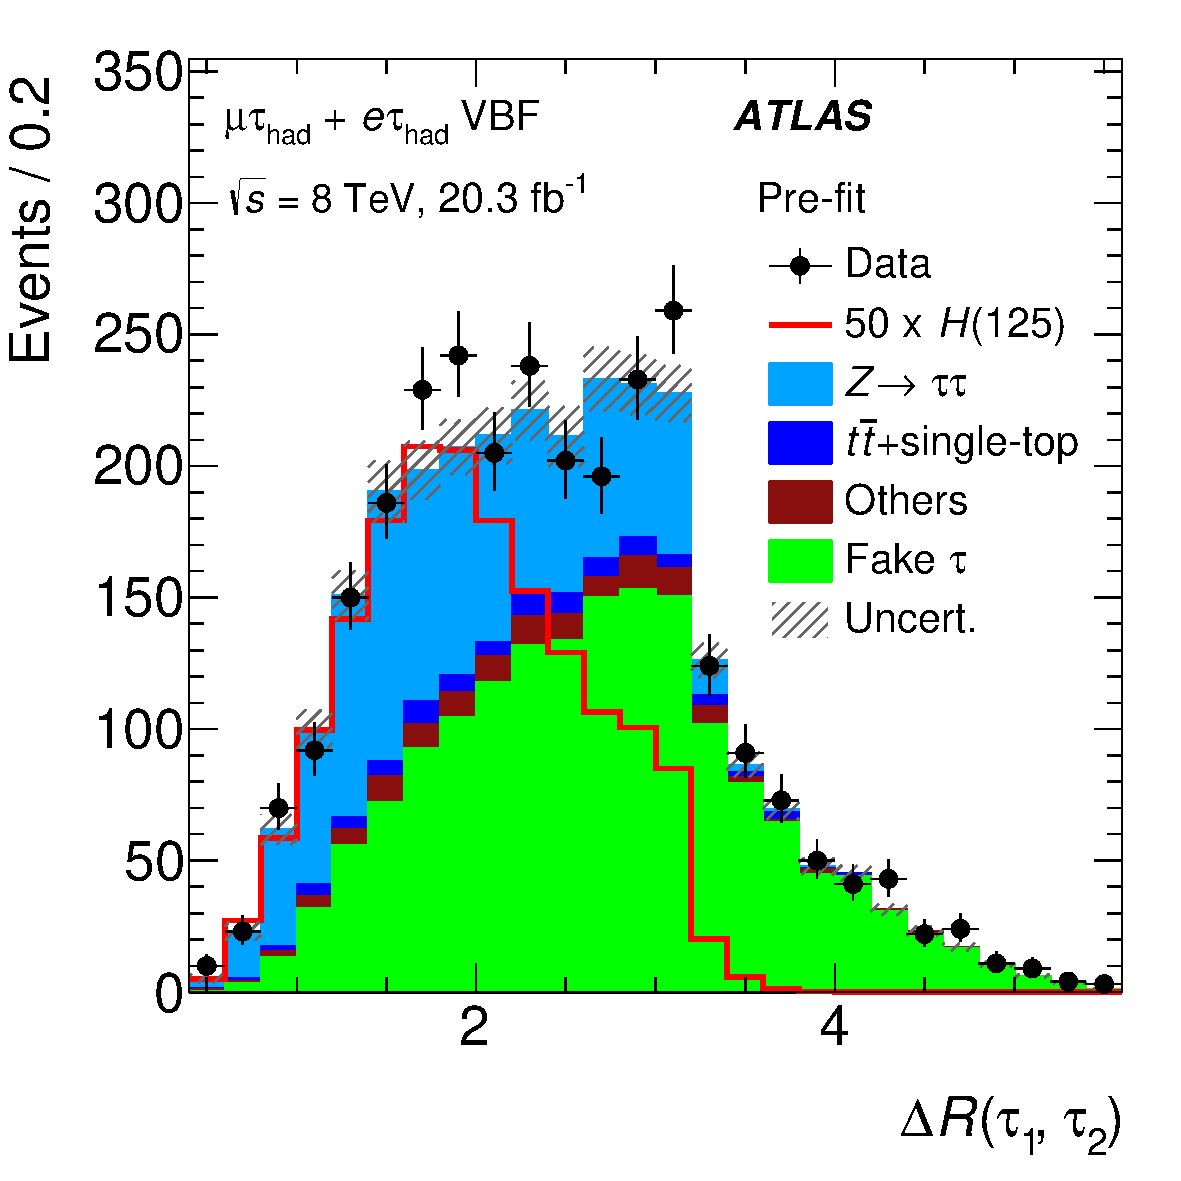
\includegraphics[width=0.30\textwidth]{figures/HIGG-2013-32/figaux_06f}
  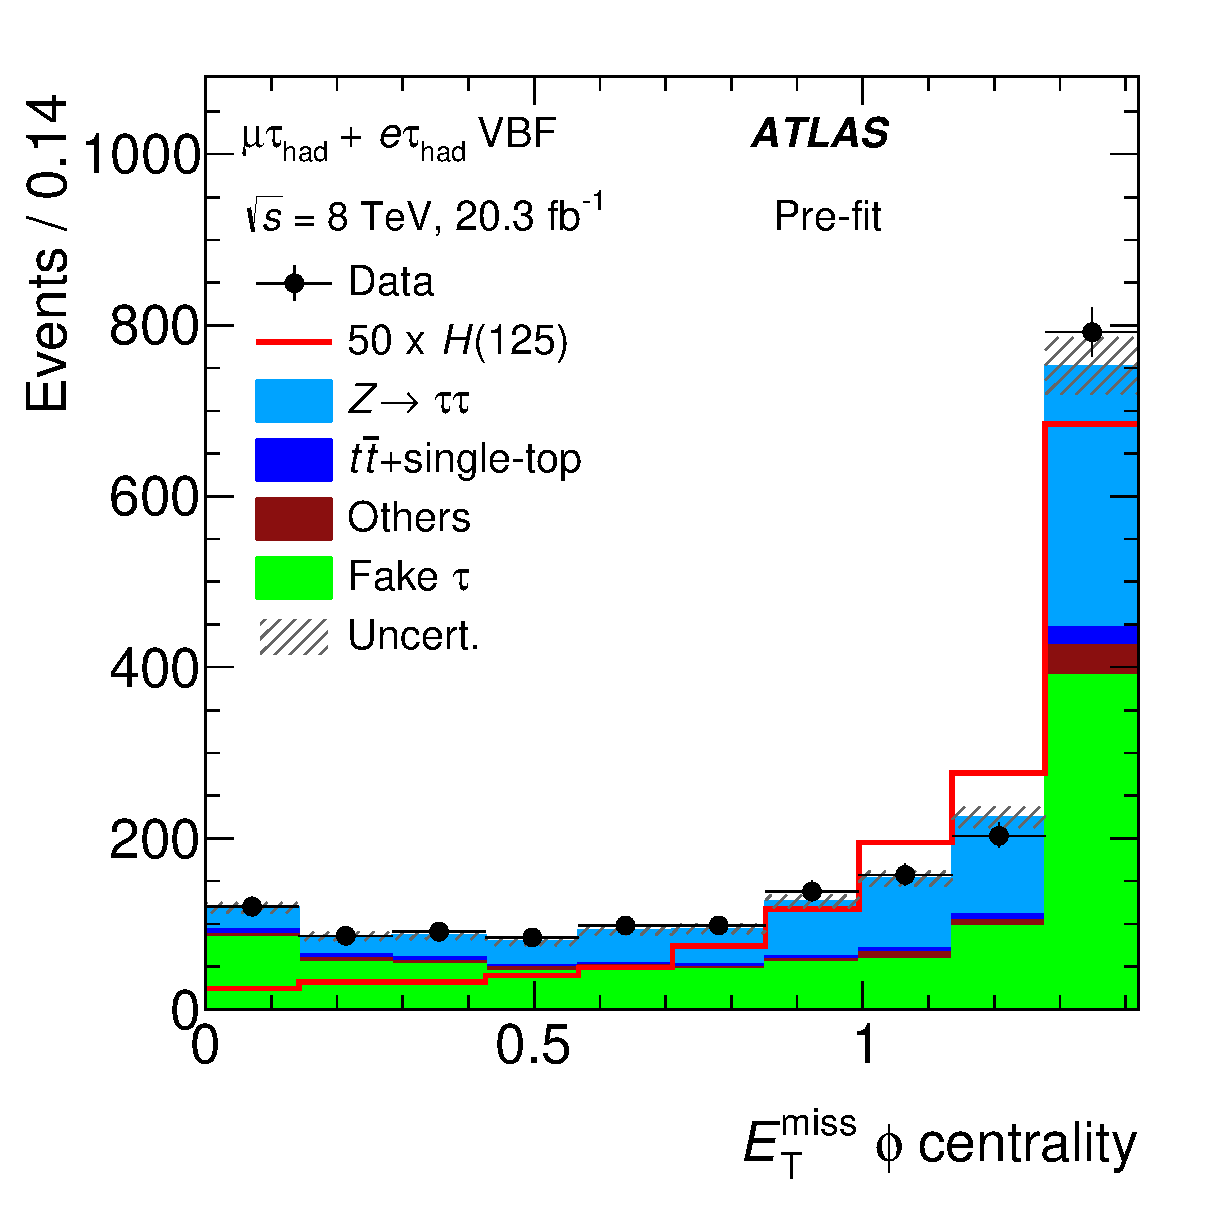
\includegraphics[width=0.30\textwidth]{figures/HIGG-2013-32/figaux_07a}
  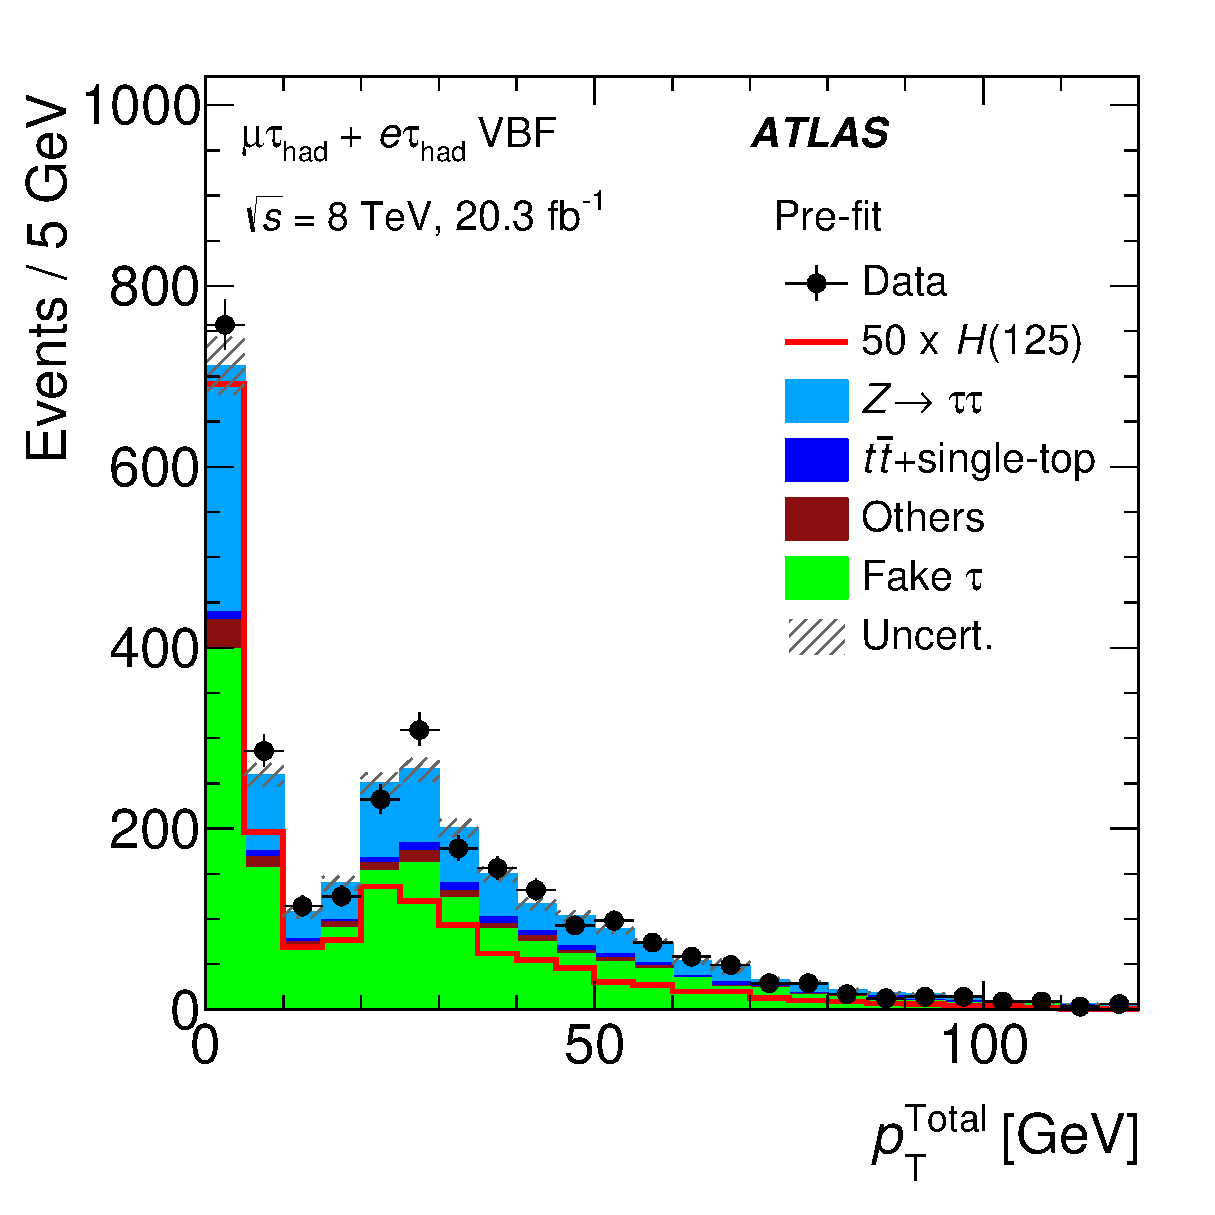
\includegraphics[width=0.30\textwidth]{figures/HIGG-2013-32/figaux_07b}
  \caption{Data and prediction for input variables to the BDT in the $\Htautaulh$ VBF signal region~\cite{HIGG-2013-32}.}
  \label{fig:results-SR-inputs}
\end{figure}

\clearpage

\begin{figure}[tp]
  \centering
  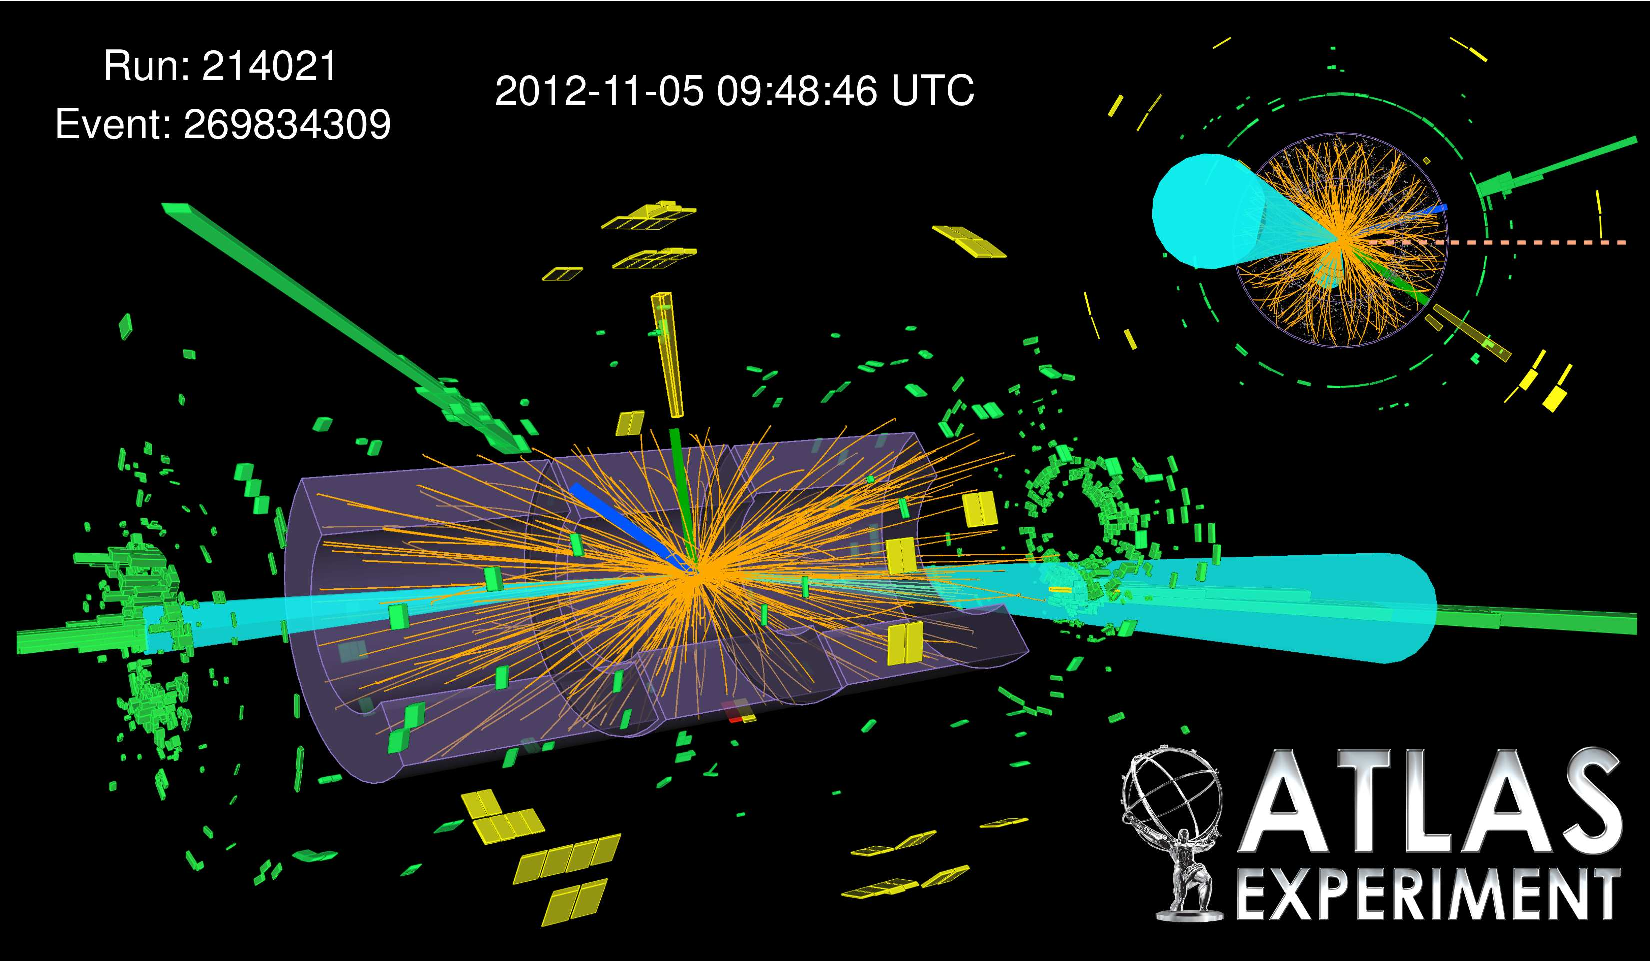
\includegraphics[width=0.90\textwidth]{figures/HIGG-2013-32/figaux_19}
  \caption{Display of one of the most signal-like events in the $\Htautaulh$ VBF category in data~\cite{HIGG-2013-32}. The blue track matched to the green cluster indicates an electron, the green track matched to the yellow cluster indicates a $\tauh$, the pink dotted line indicates the $\MET$ in the transverse plane, and the turquoise cones indicates the VBF jets. The reconstructed $\mMMC = 127$ GeV and $\mjj = 1.53$ TeV.}
  \label{fig:results-eventdisplay}
\end{figure}

\section{$\Htautauhh$ and $\Htautaull$}
\label{sec:results-hhll}

\begin{figure}[tp]
  \centering
  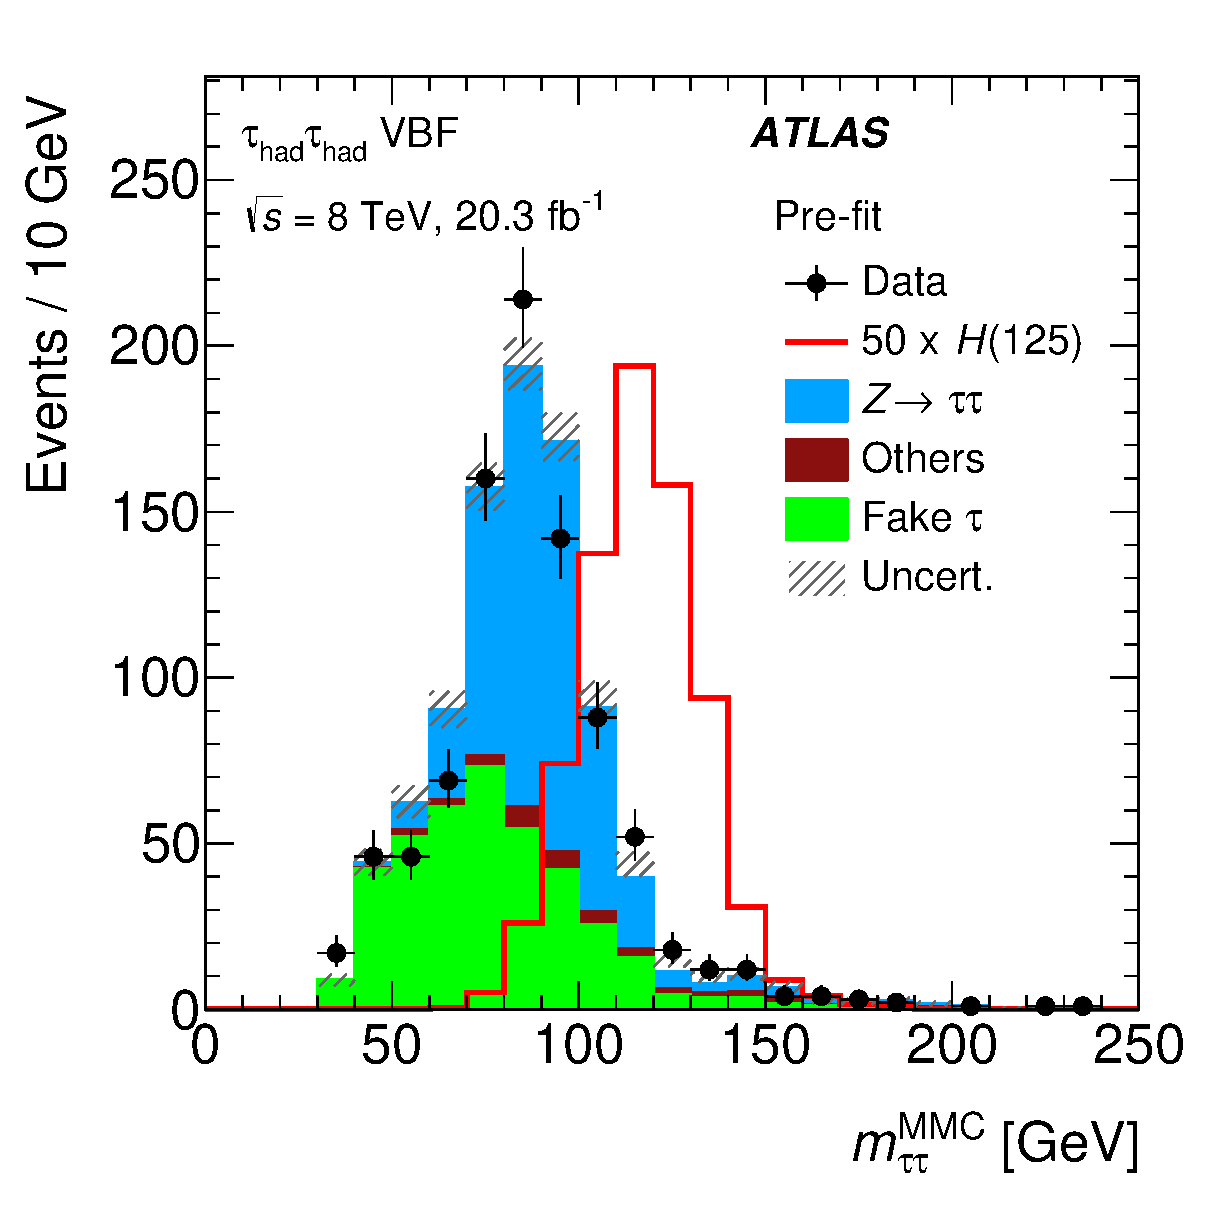
\includegraphics[width=0.48\textwidth]{figures/HIGG-2013-32/figaux_09d}
  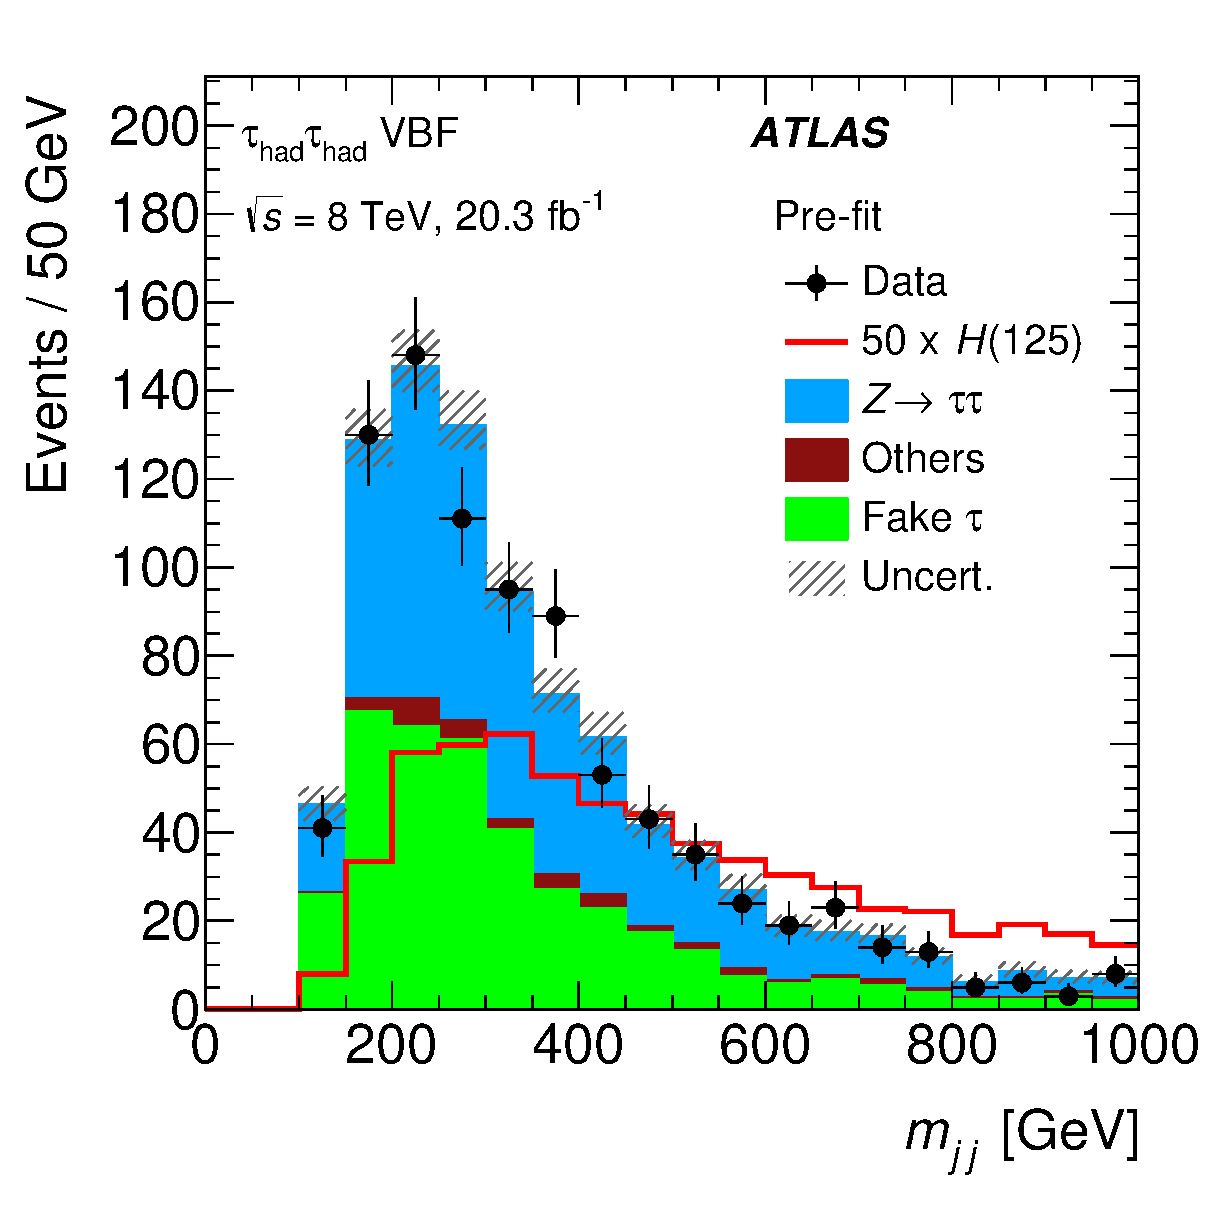
\includegraphics[width=0.48\textwidth]{figures/HIGG-2013-32/figaux_09c}
  \caption{Two of the nine input variables to the VBF $\Htautauhh$ BDT discriminator: $\mMMC$ (left) and $\mjj$ (right).~\cite{HIGG-2013-32}.}
  \label{fig:results-inputs-hadhad}
\end{figure}

\begin{figure}[tp]
  \centering
  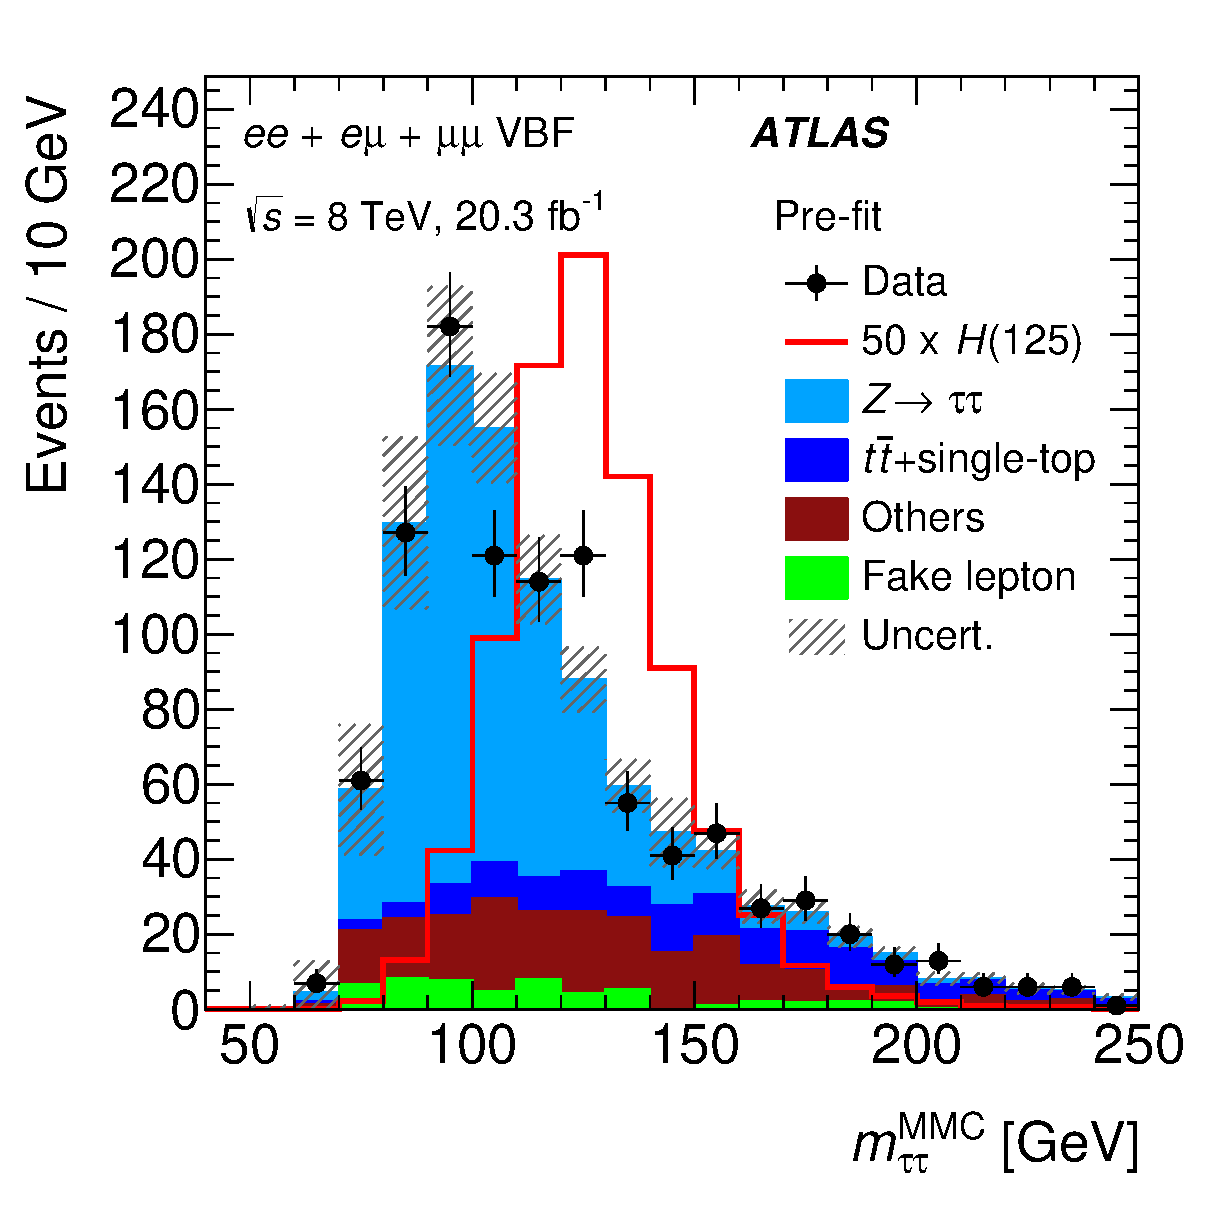
\includegraphics[width=0.48\textwidth]{figures/HIGG-2013-32/figaux_03c}
  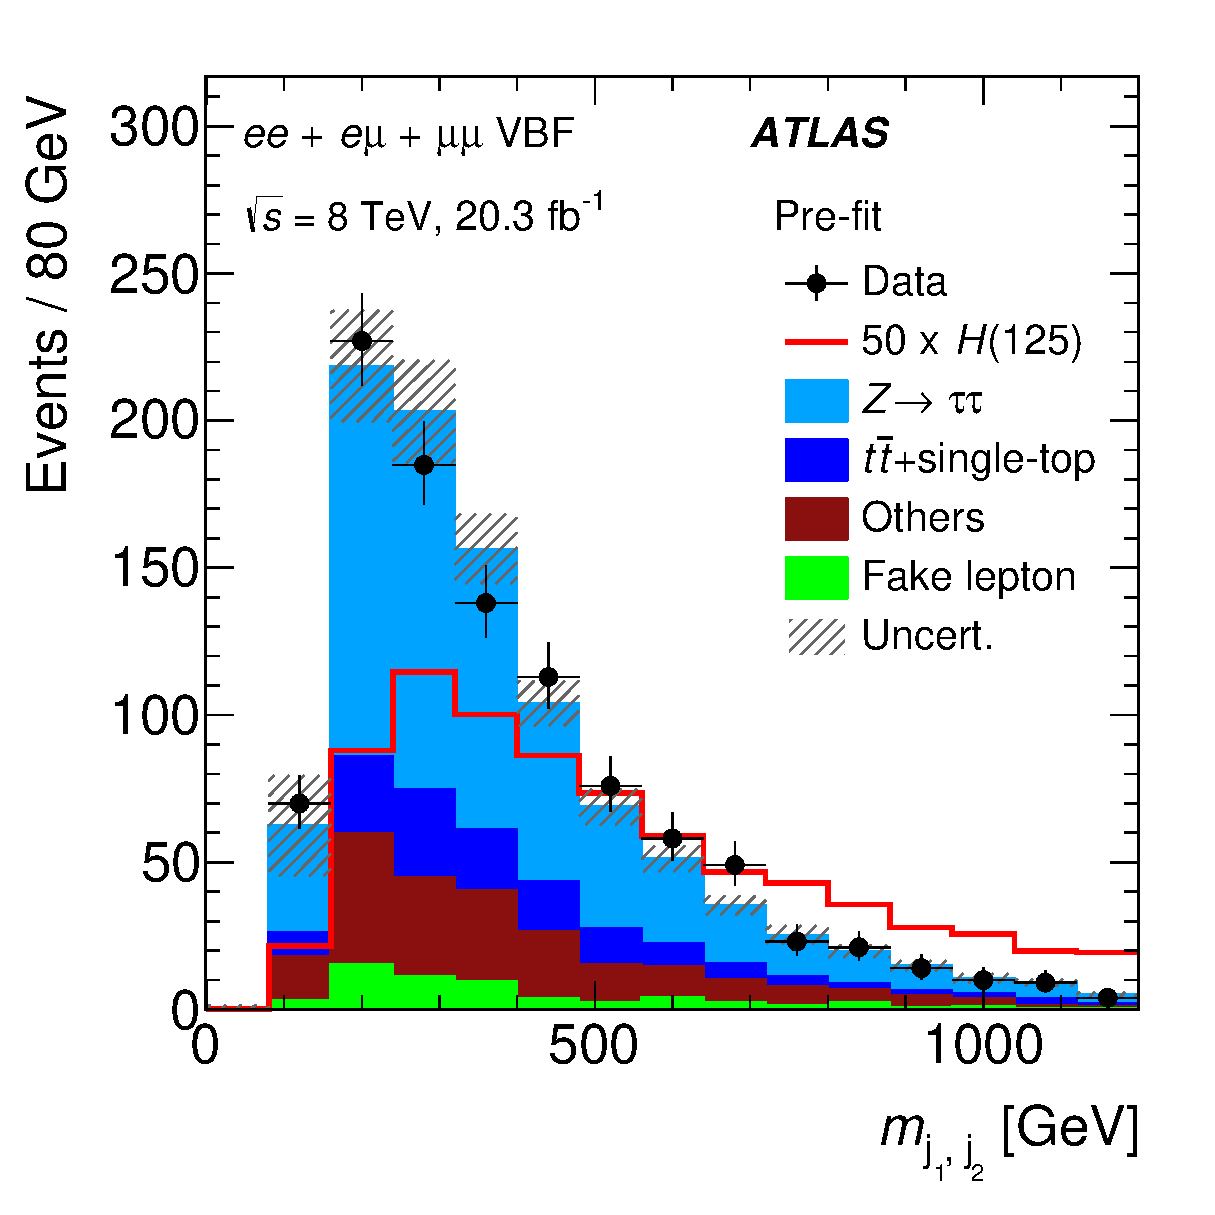
\includegraphics[width=0.48\textwidth]{figures/HIGG-2013-32/figaux_03b}
  \caption{Two of the seven input variables to the VBF $\Htautaull$ BDT discriminator: $\mMMC$ (left) and $\mjj$ (right).~\cite{HIGG-2013-32}.}
  \label{fig:results-inputs-hadhad}
\end{figure}

\section{Fit procedure}
\label{sec:results-fit-procedure}

\section{Fit results}
\label{sec:results-fit-results}

\clearpage

\begin{figure}[tp]
  \centering
  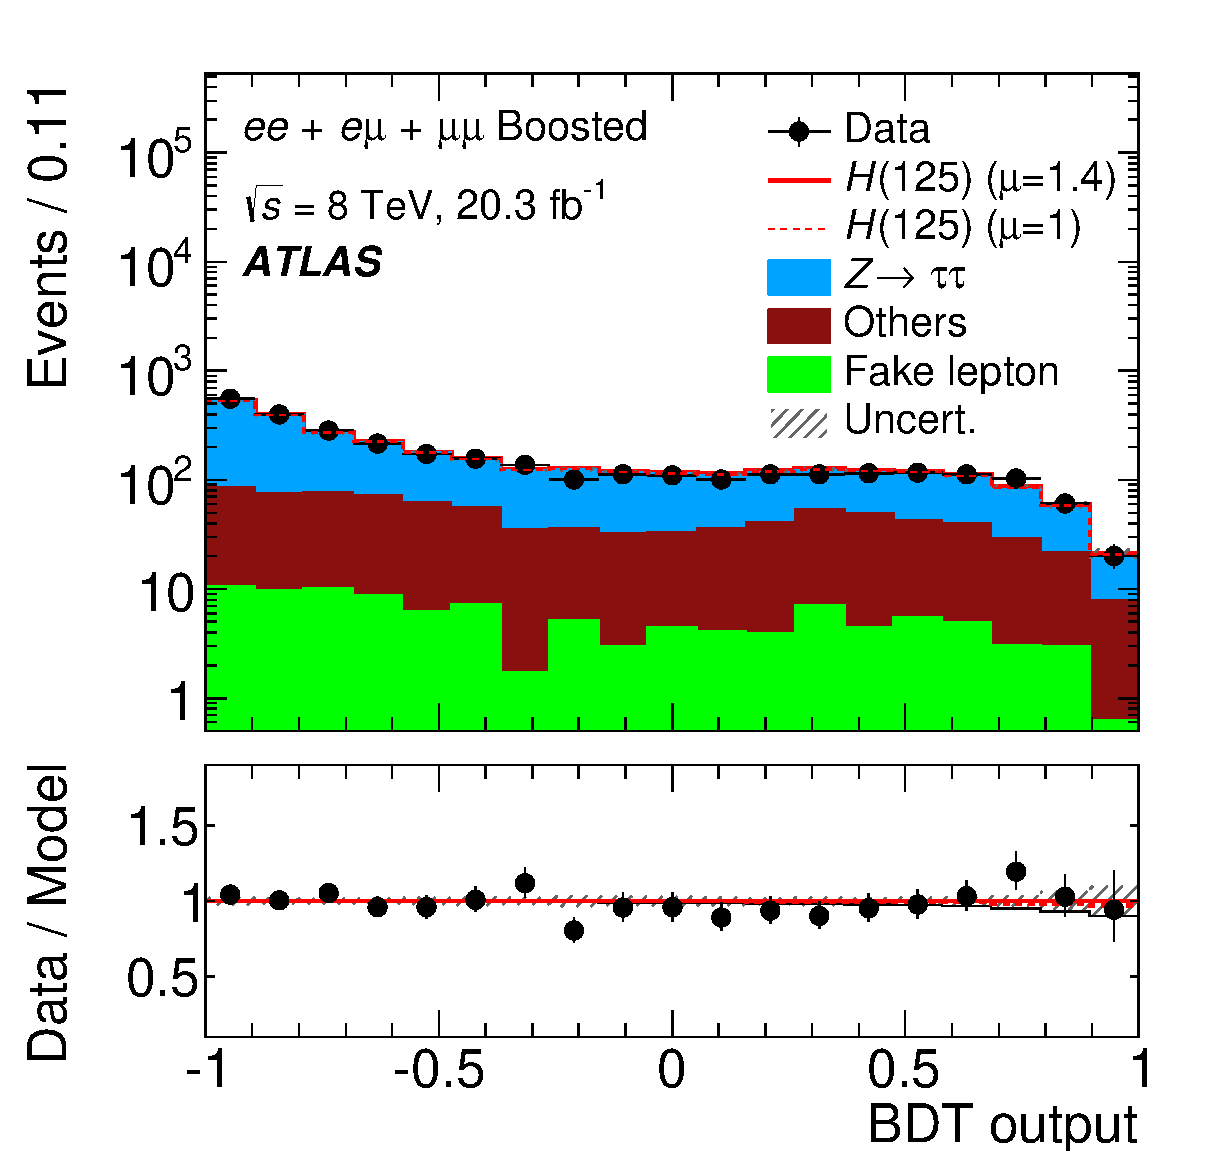
\includegraphics[width=0.48\textwidth]{figures/HIGG-2013-32/fig_08b}
  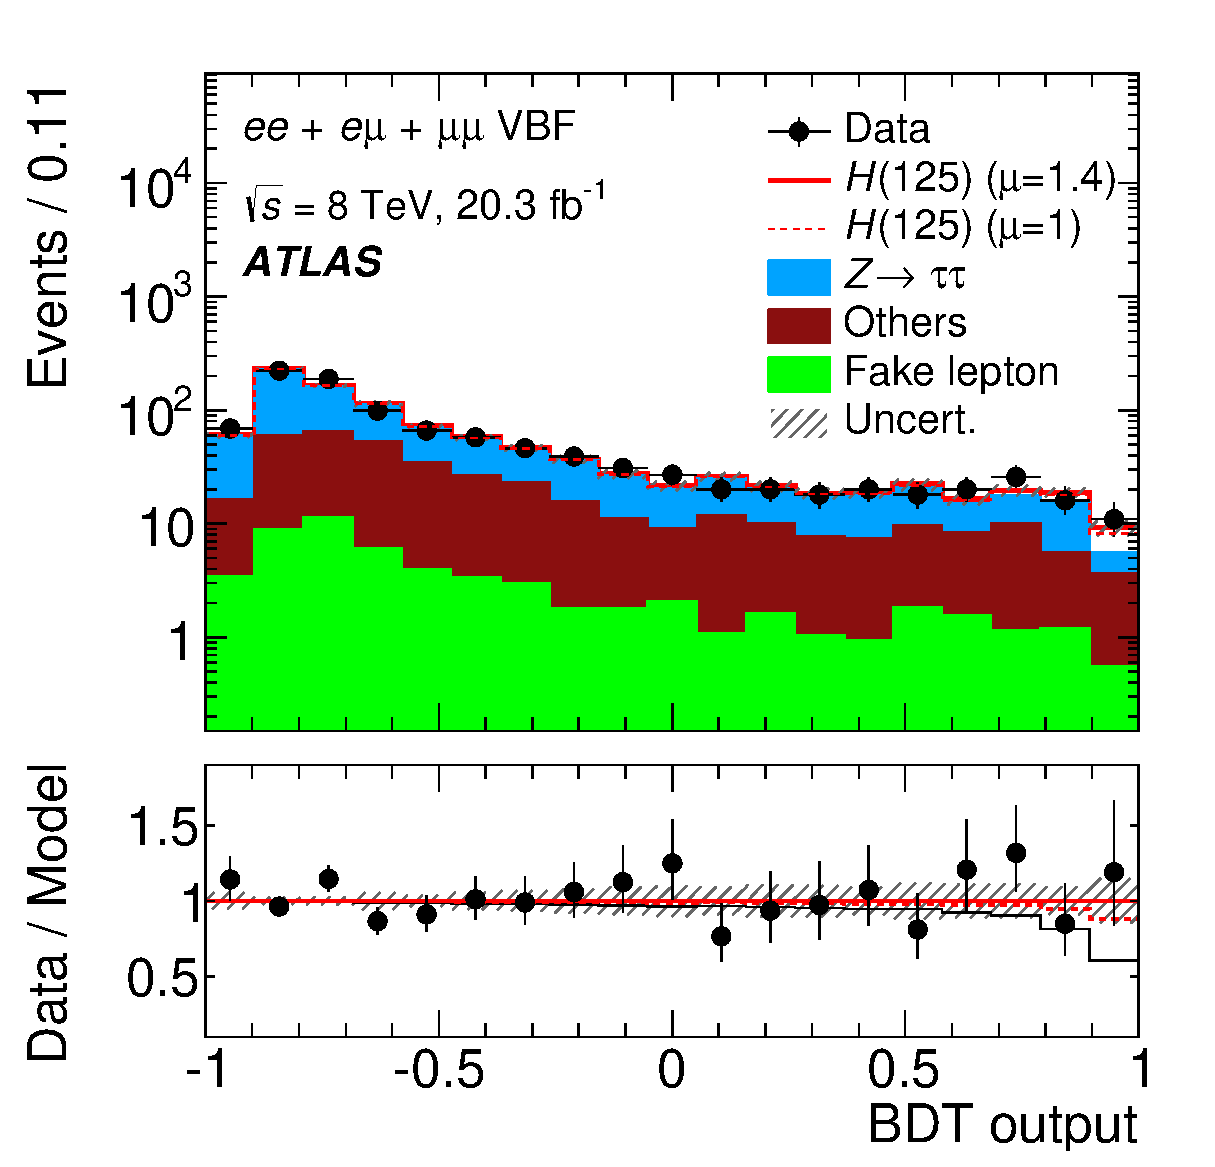
\includegraphics[width=0.48\textwidth]{figures/HIGG-2013-32/fig_08a}
  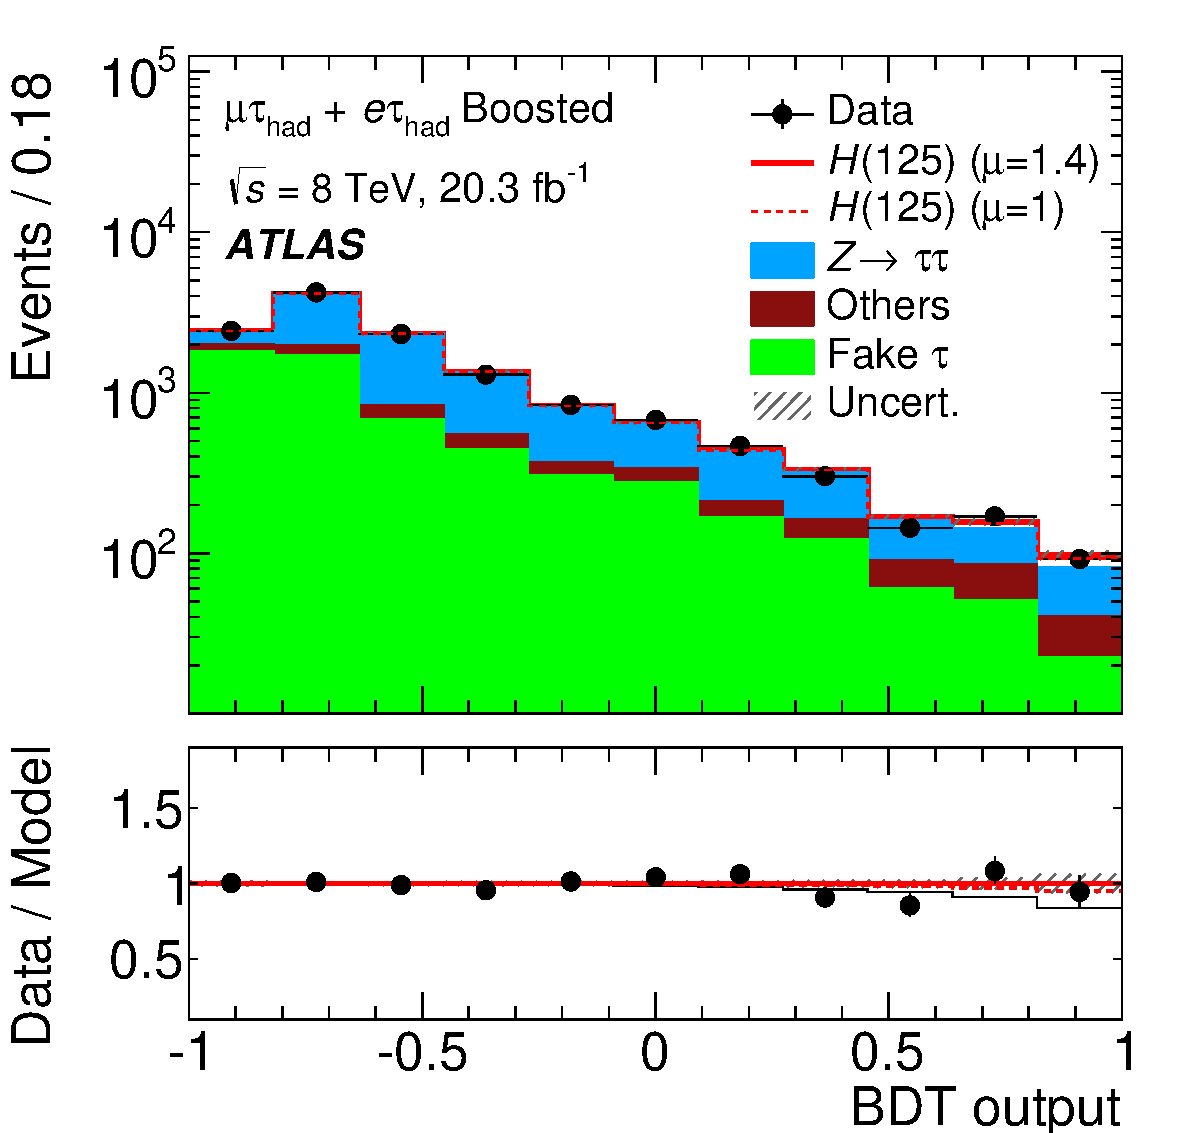
\includegraphics[width=0.48\textwidth]{figures/HIGG-2013-32/fig_08d}
  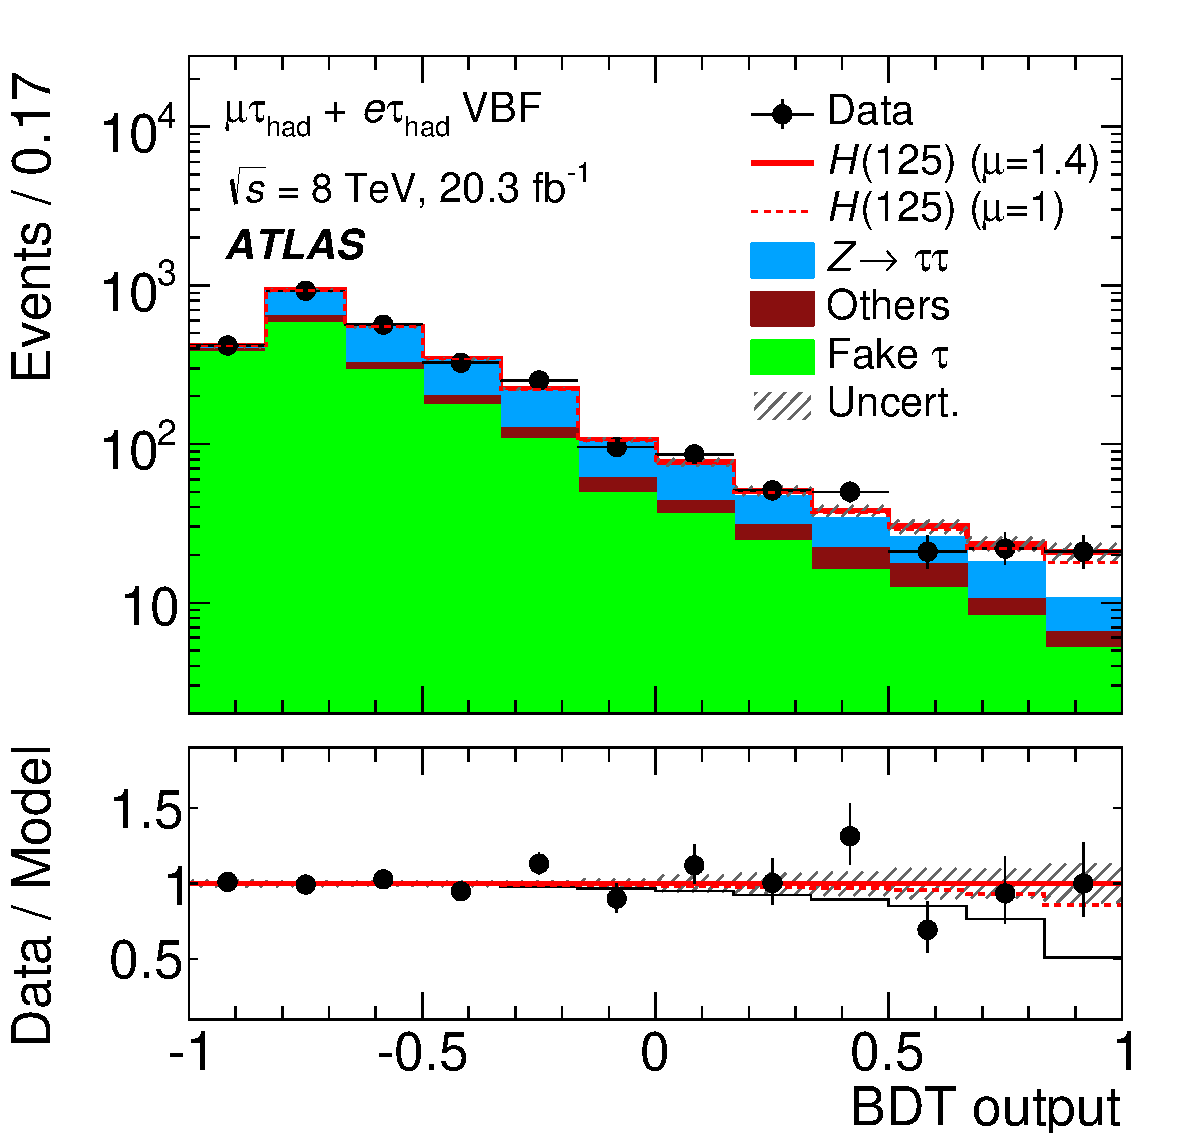
\includegraphics[width=0.48\textwidth]{figures/HIGG-2013-32/fig_08c}
  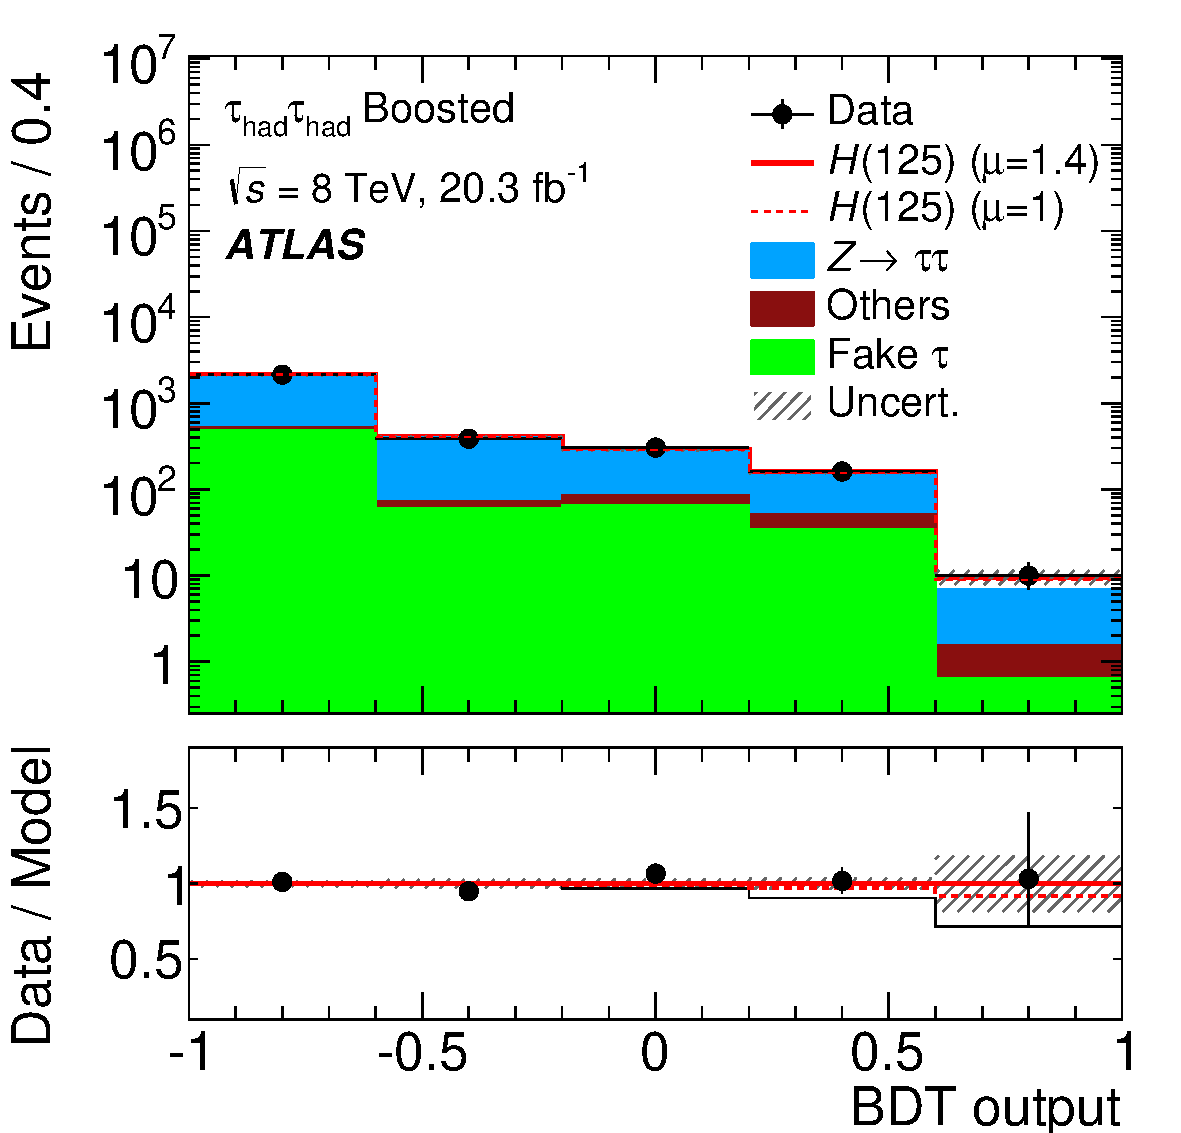
\includegraphics[width=0.48\textwidth]{figures/HIGG-2013-32/fig_08f}
  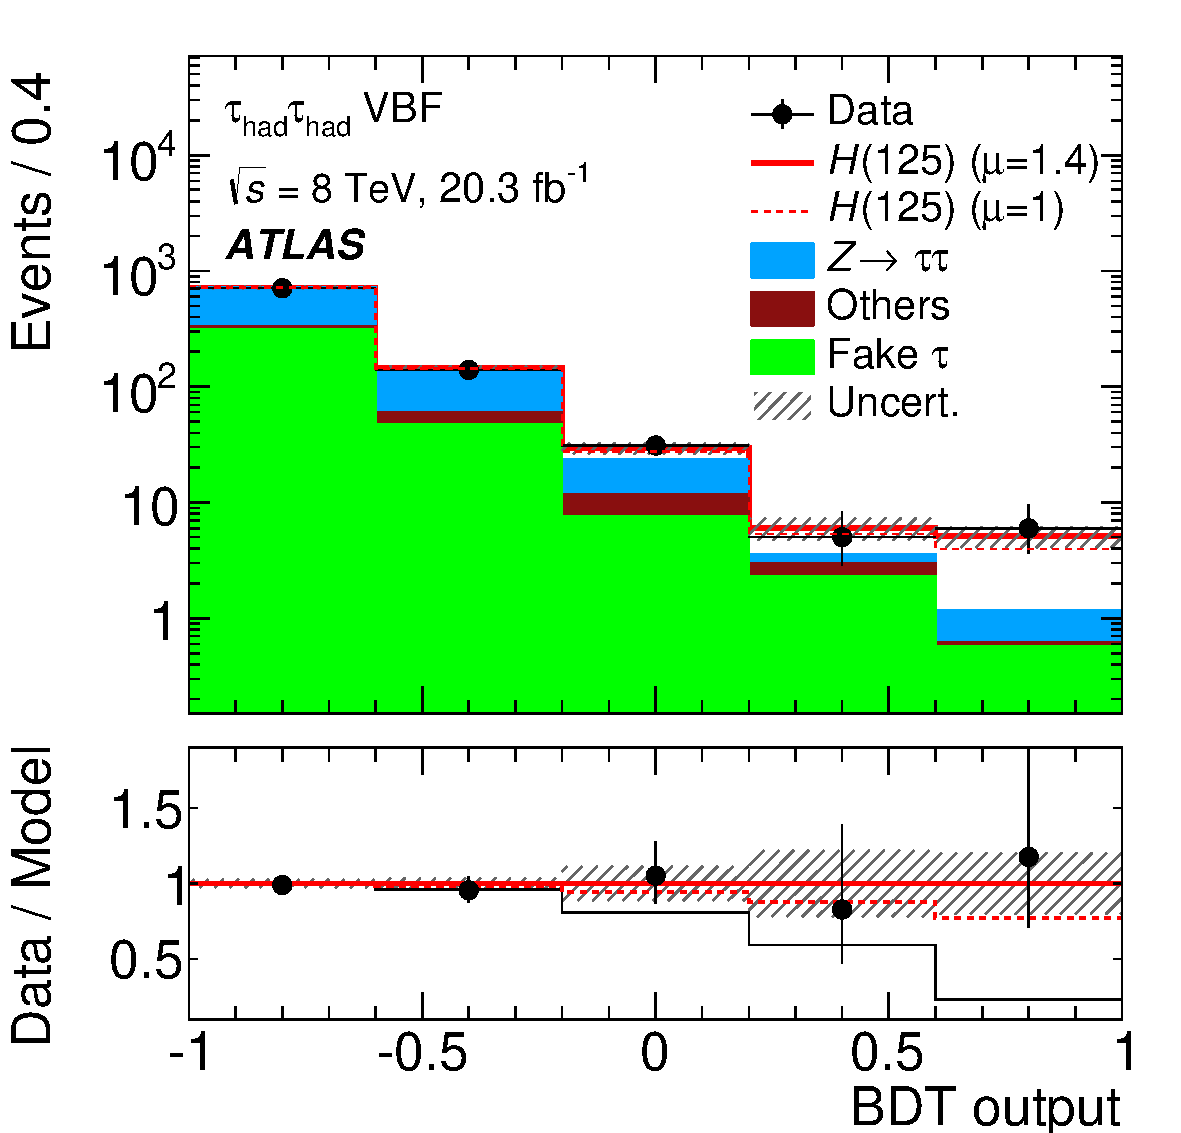
\includegraphics[width=0.48\textwidth]{figures/HIGG-2013-32/fig_08e}
  \caption{Distributions of the 8 TeV BDT discriminants in all six analysis categories after the global fit~\cite{HIGG-2013-32}.}
  \label{fig:results-bdts}
\end{figure}

\clearpage

\begin{figure}[tp]
  \centering
  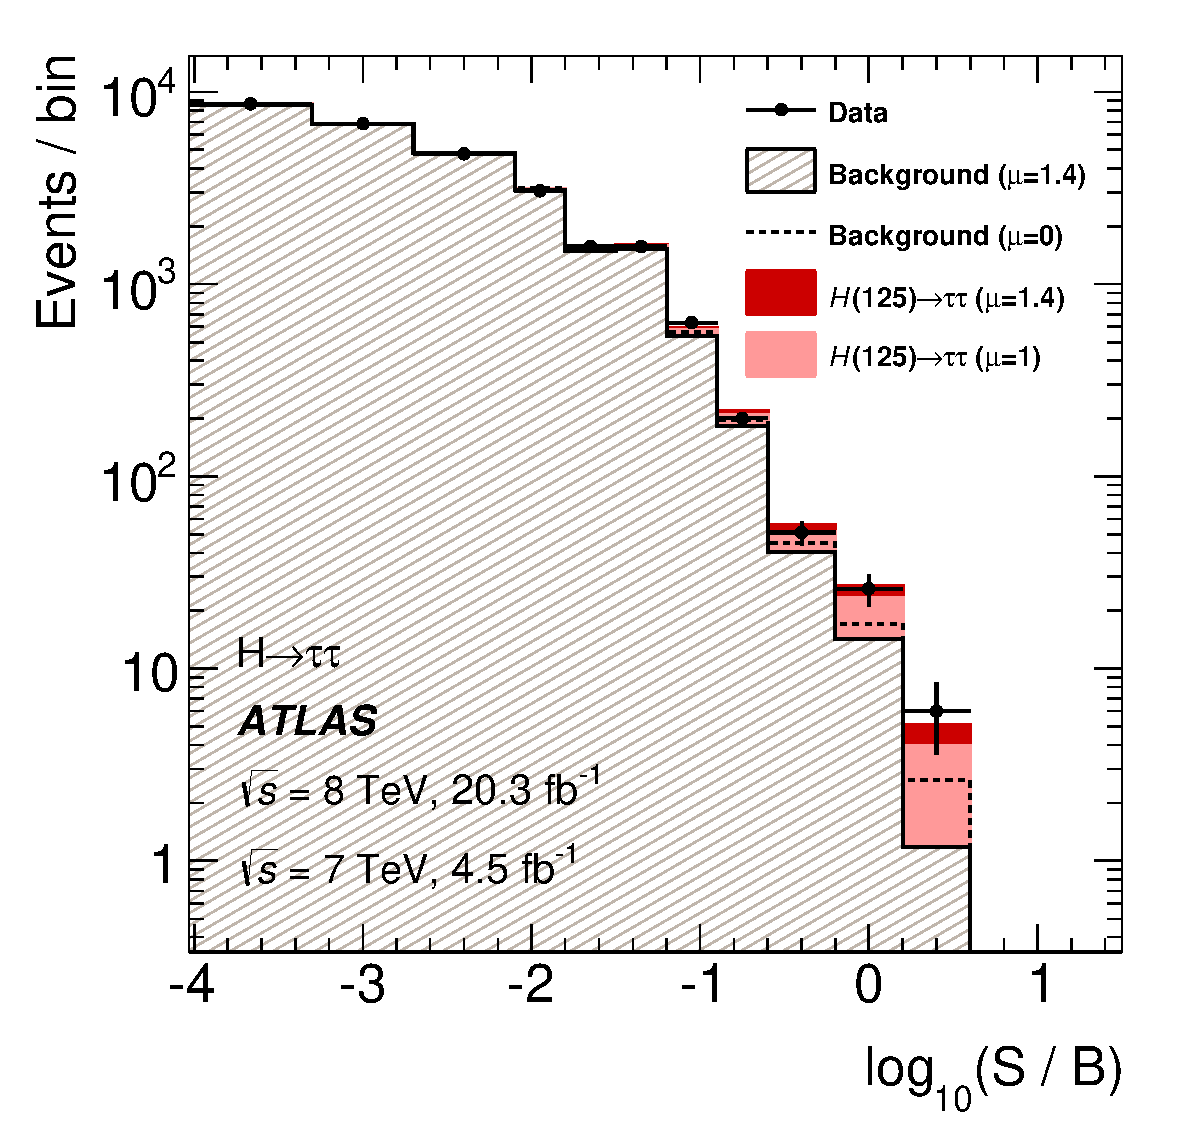
\includegraphics[width=0.48\textwidth]{figures/HIGG-2013-32/fig_10}
  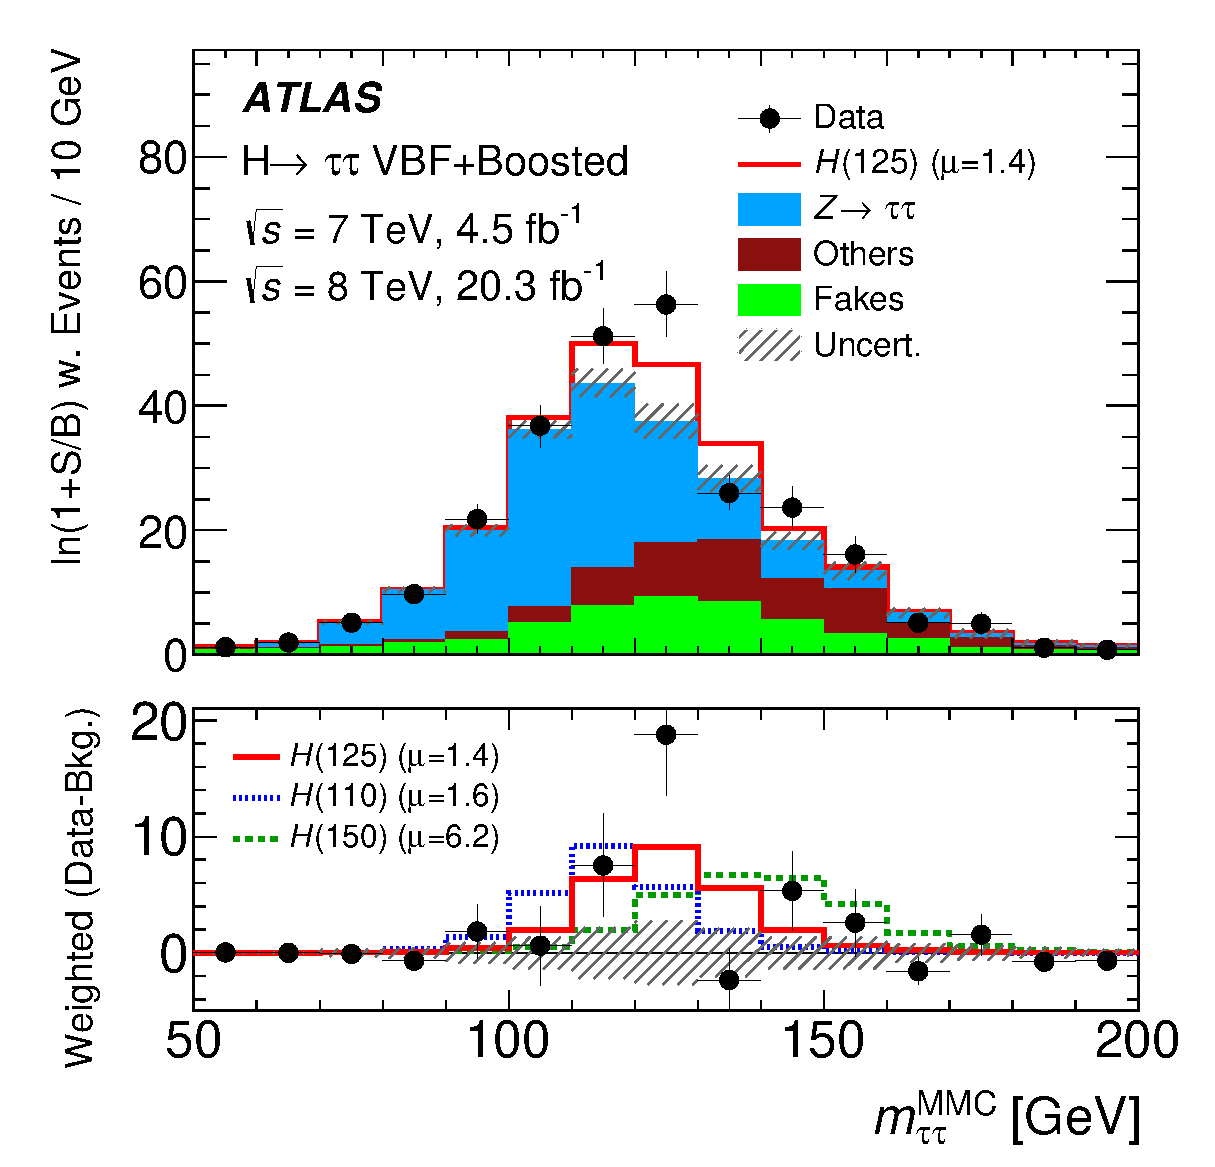
\includegraphics[width=0.48\textwidth]{figures/HIGG-2013-32/fig_11b}
  \caption{Plots of data and prediction which emphasize the most sensitive regions~\cite{HIGG-2013-32}. The individual BDT bins from all six categories are ordered by S/B and plotted on a shared axis (left) and entries in the $\mMMC$ distribution are weighted by $\text{log}(1+S/B)$ (right).}
  \label{fig:results-money-plots}
\end{figure}

\begin{figure}[tp]
  \centering
  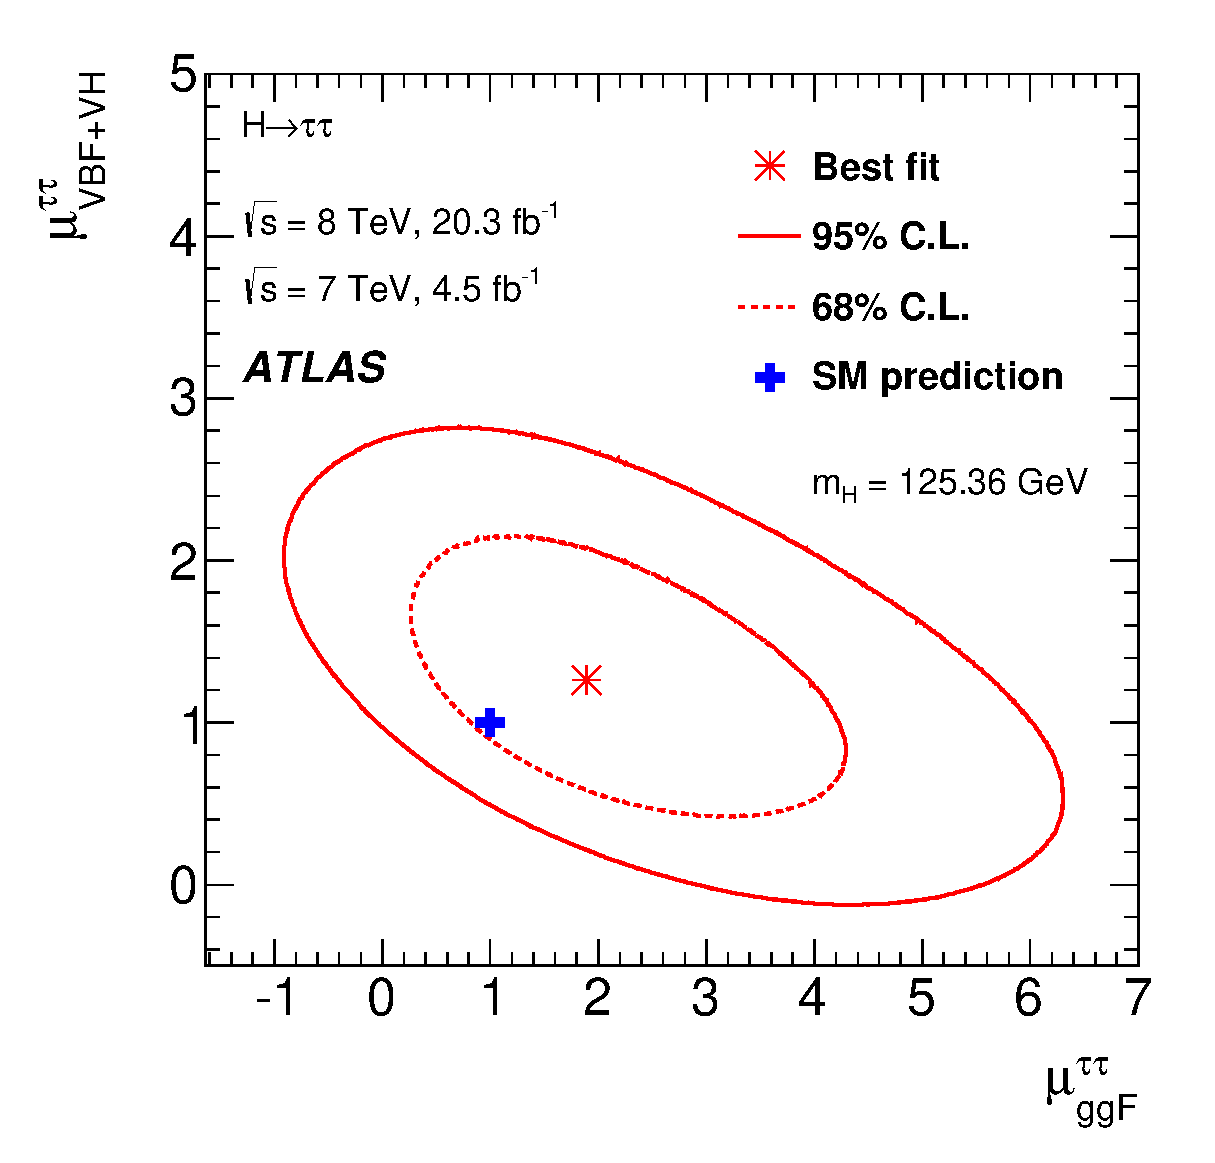
\includegraphics[width=0.48\textwidth]{figures/HIGG-2013-32/fig_12}
  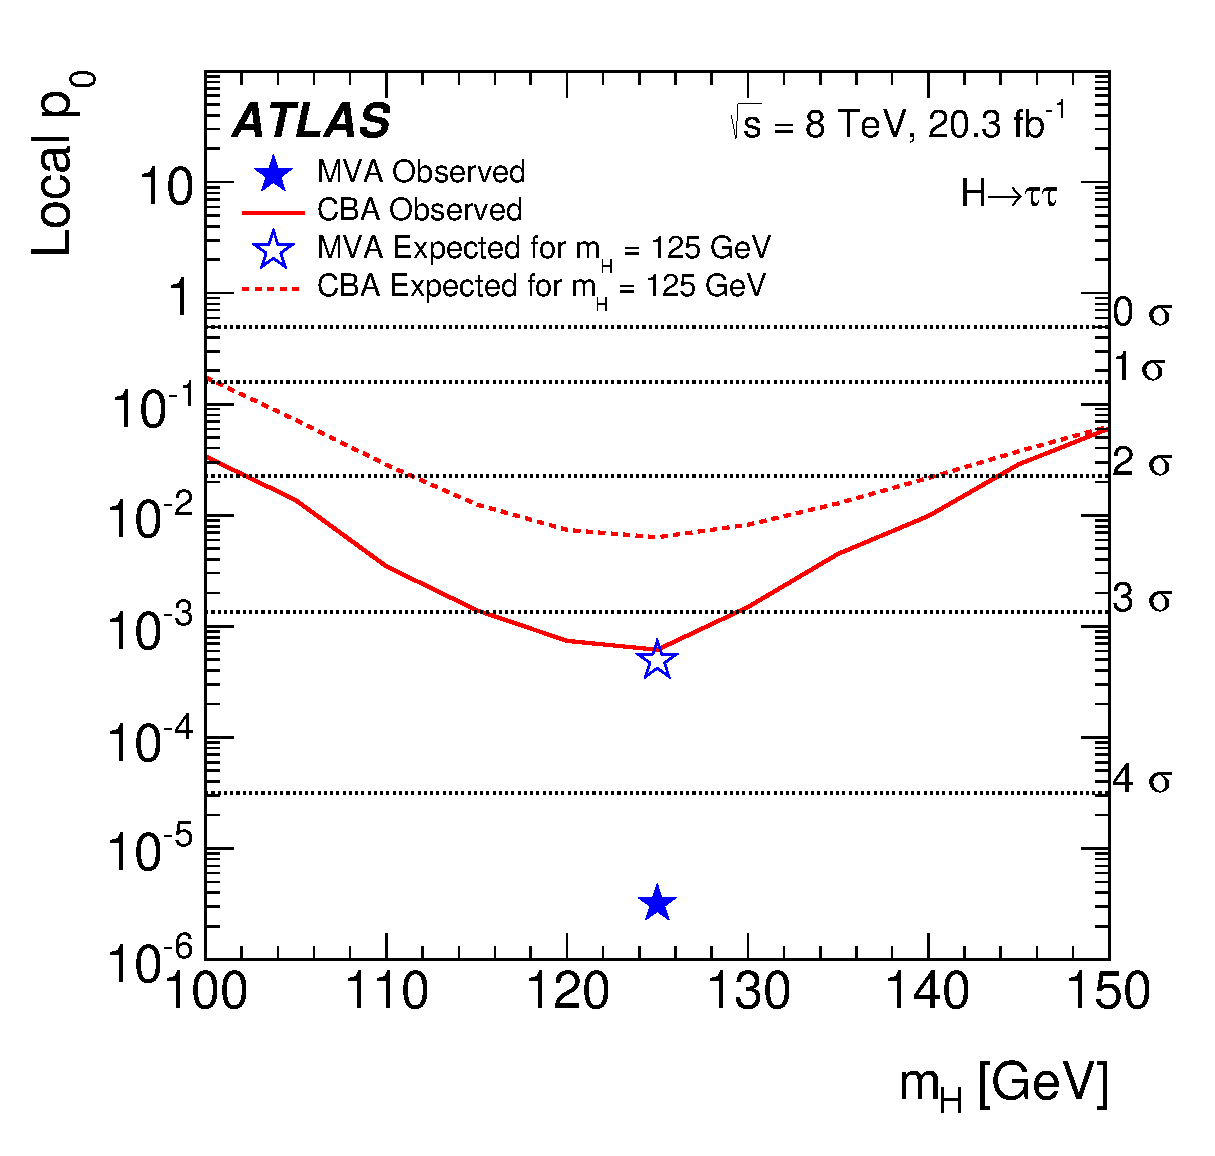
\includegraphics[width=0.48\textwidth]{figures/HIGG-2013-32/fig_14}
  \caption{Two-dimensional contours of the fitted signal strength $\mu$ comparing VBF and ggF production mechanisms (left) and the local $p_0$ for the MVA and cuts-based analyses as a function of the Higgs mass hypothesis (right)~\cite{HIGG-2013-32}.}
  \label{fig:results-mup0}
\end{figure}

\begin{figure}[tp]
  \centering
  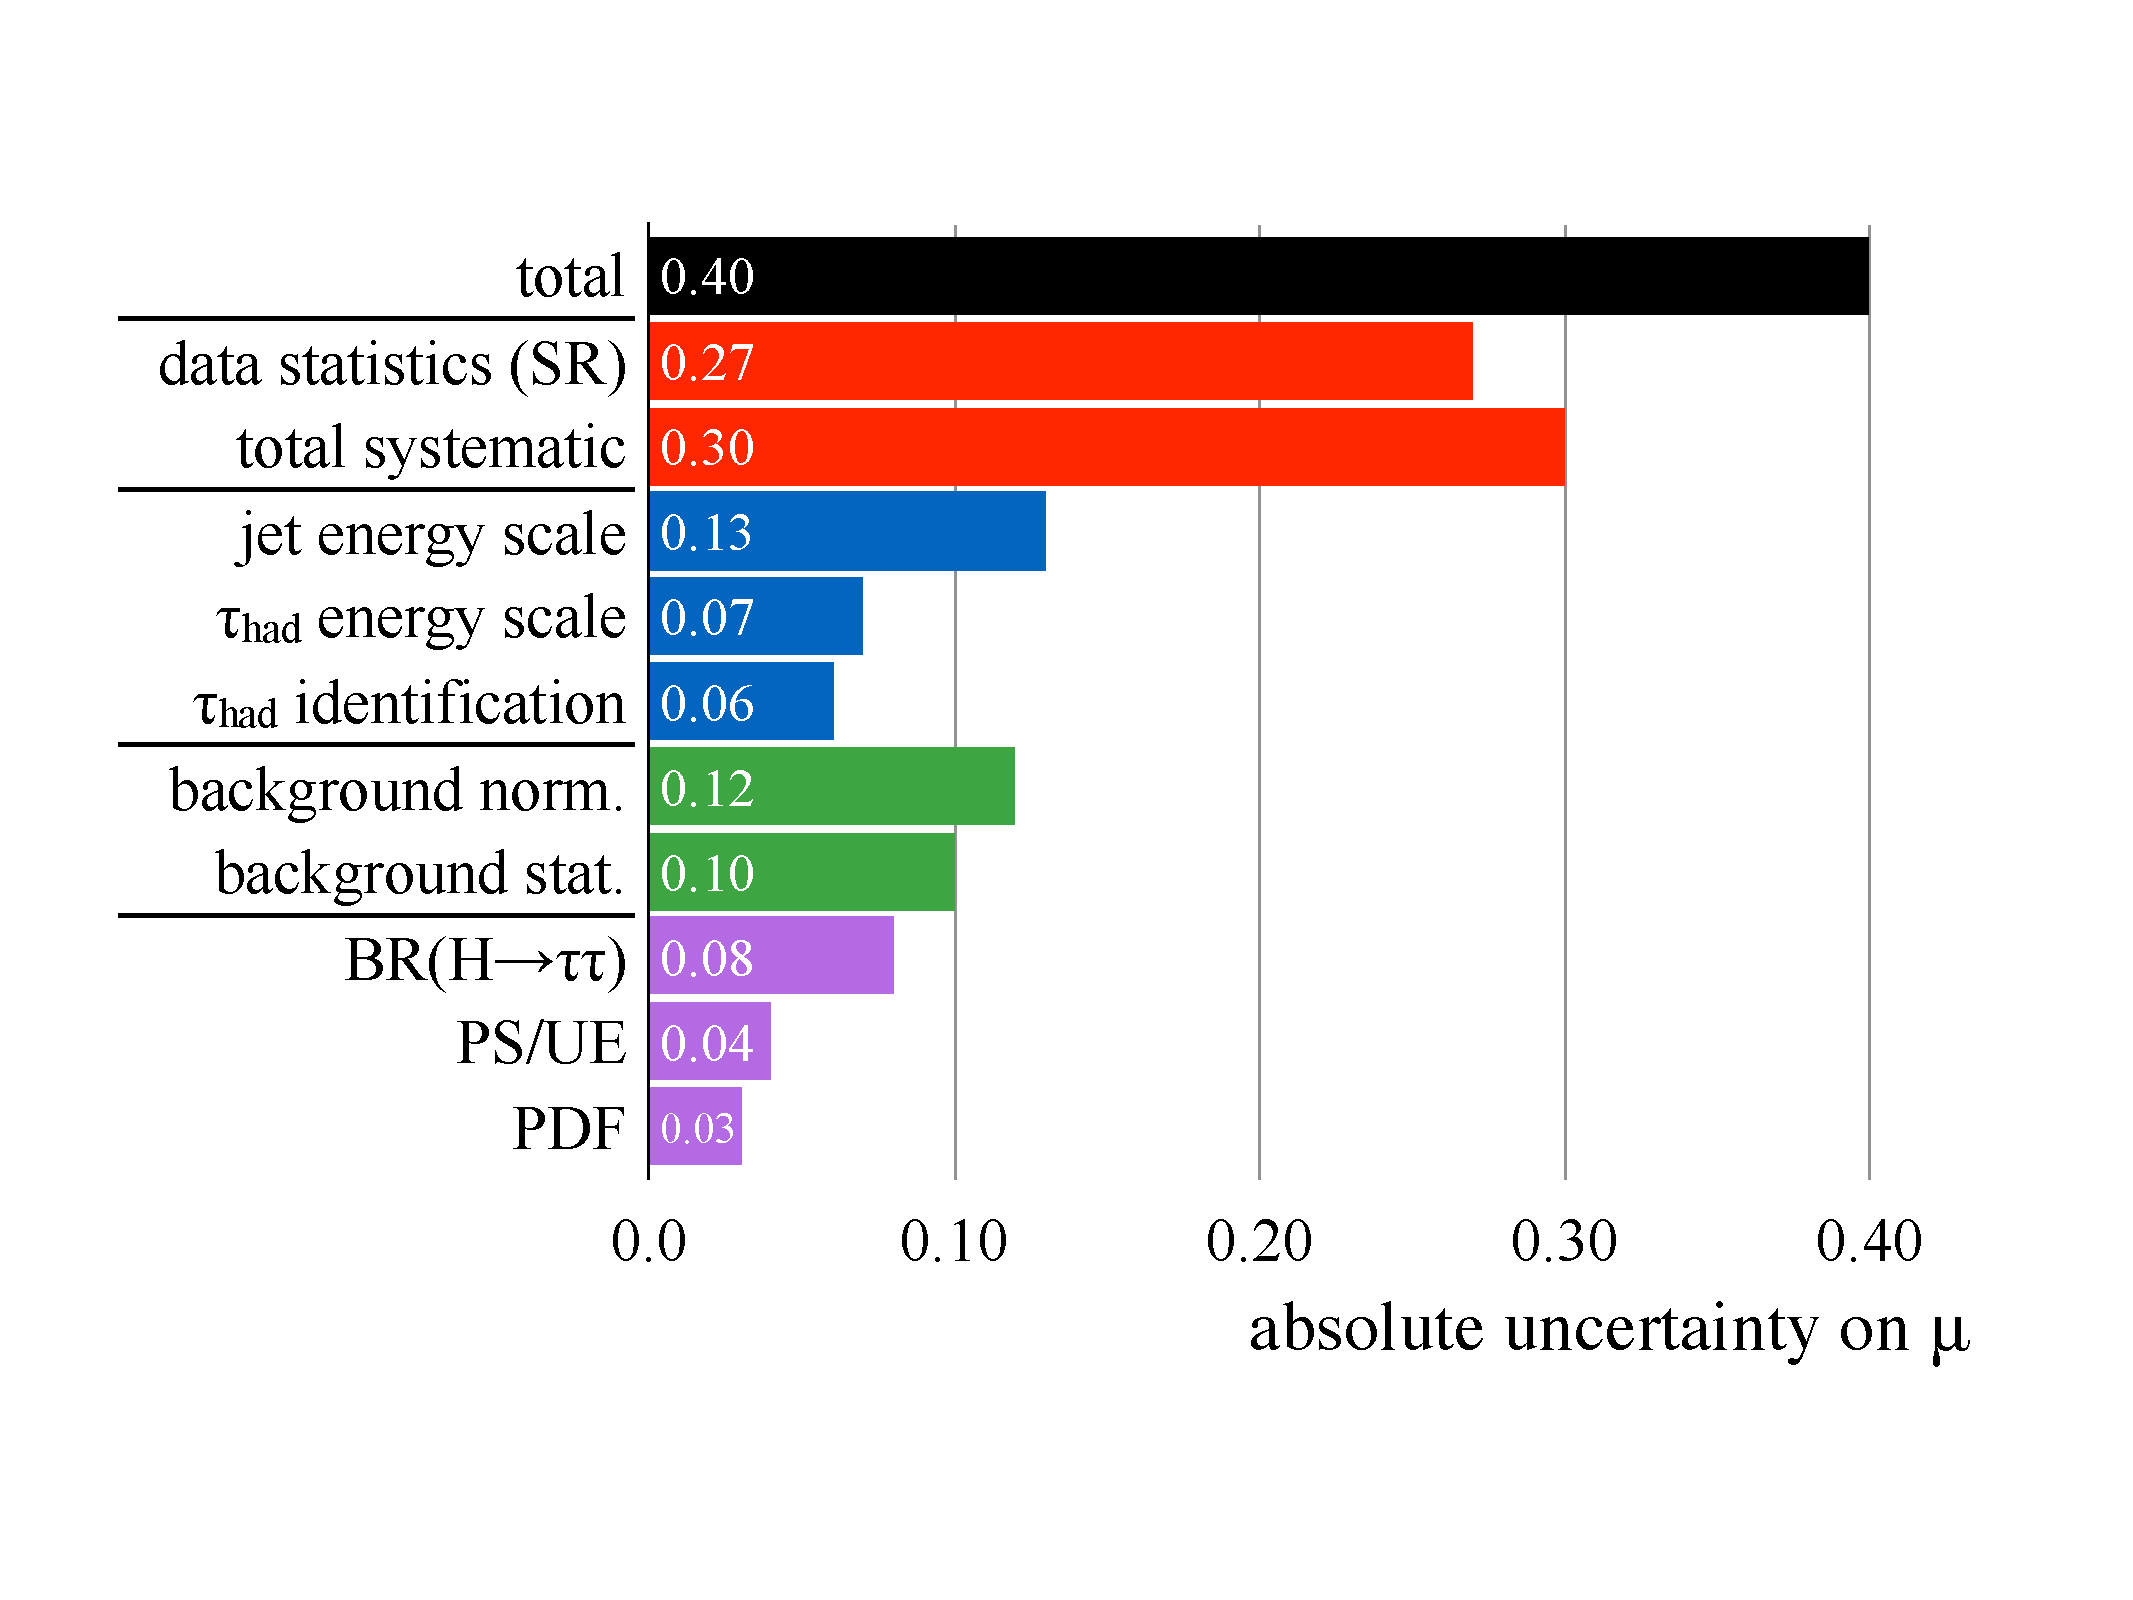
\includegraphics[width=0.90\textwidth]{figures/HIGG-2013-32/uncertainties}
  \caption{Comparison of the impact of the statistical and systematic uncertainties on the absolute uncertainty on $\mu$~\cite{HIGG-2013-32}.}
  \label{fig:results-uncertainties-1}
\end{figure}

\clearpage

\begin{figure}[tp]
  \centering
  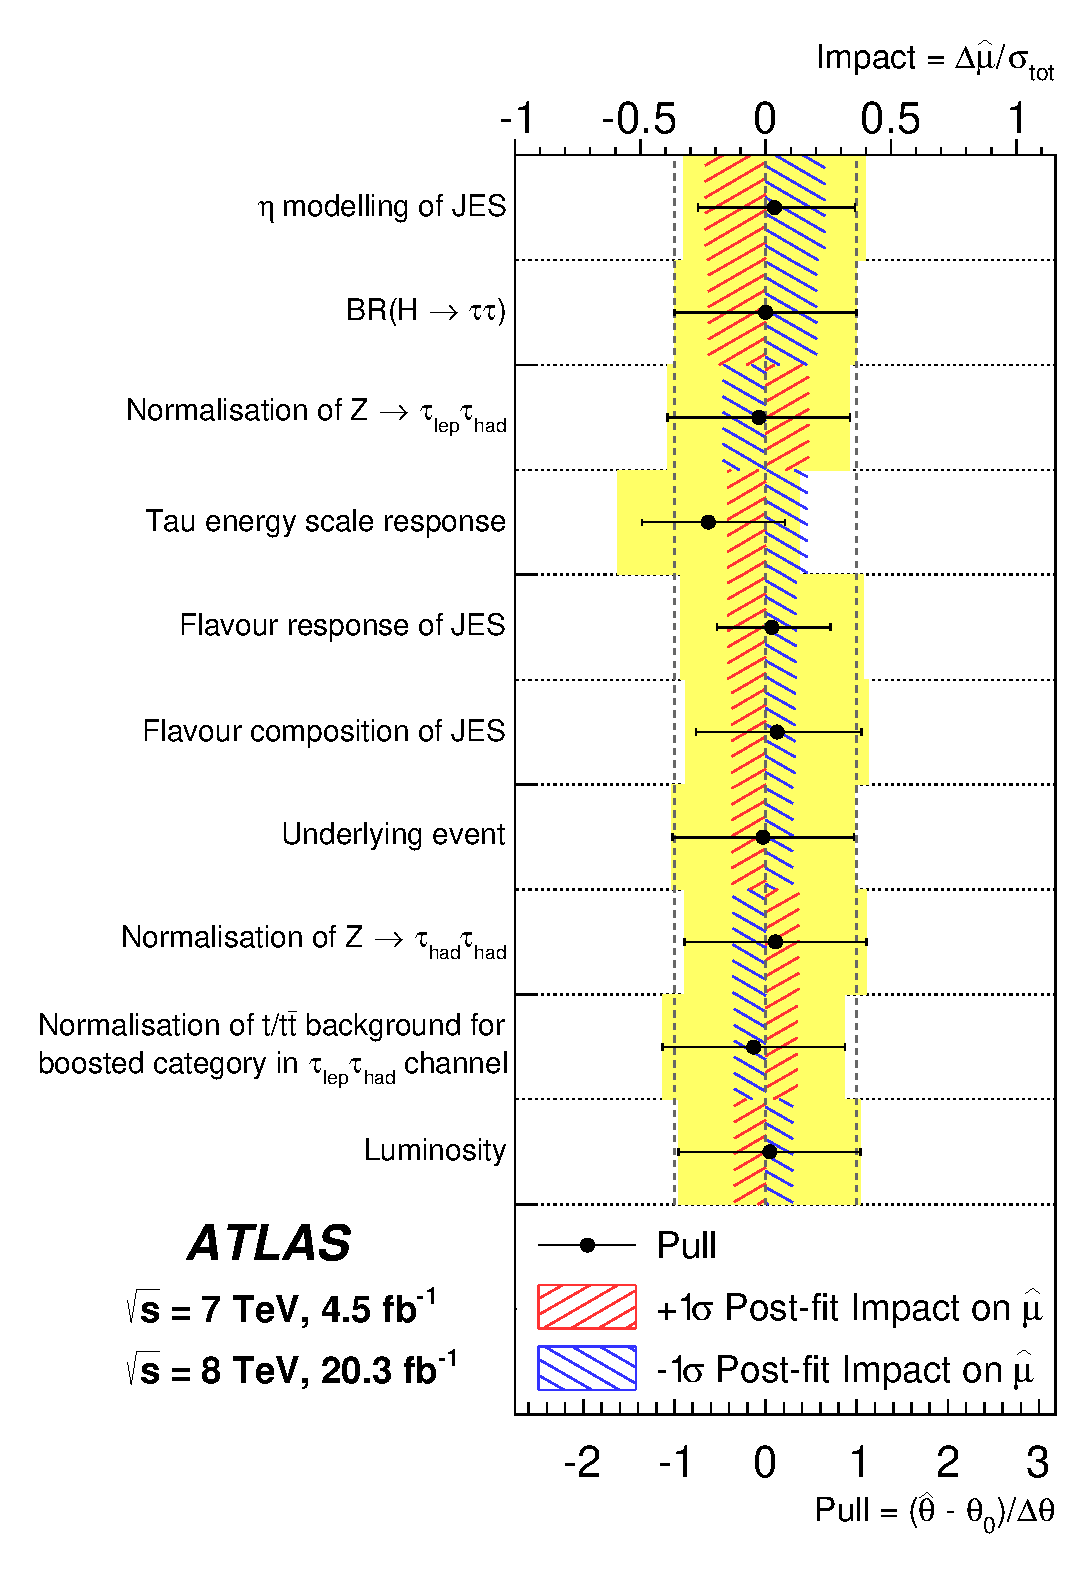
\includegraphics[width=0.90\textwidth]{figures/HIGG-2013-32/fig_07}
  \caption{Comparison of the impact and pull of the dominant individual systematic uncertainties on the absolute uncertainty on $\mu$~\cite{HIGG-2013-32}.}
  \label{fig:results-uncertainties-2}
\end{figure}

\clearpage

\begin{figure}[tp]
  \centering
  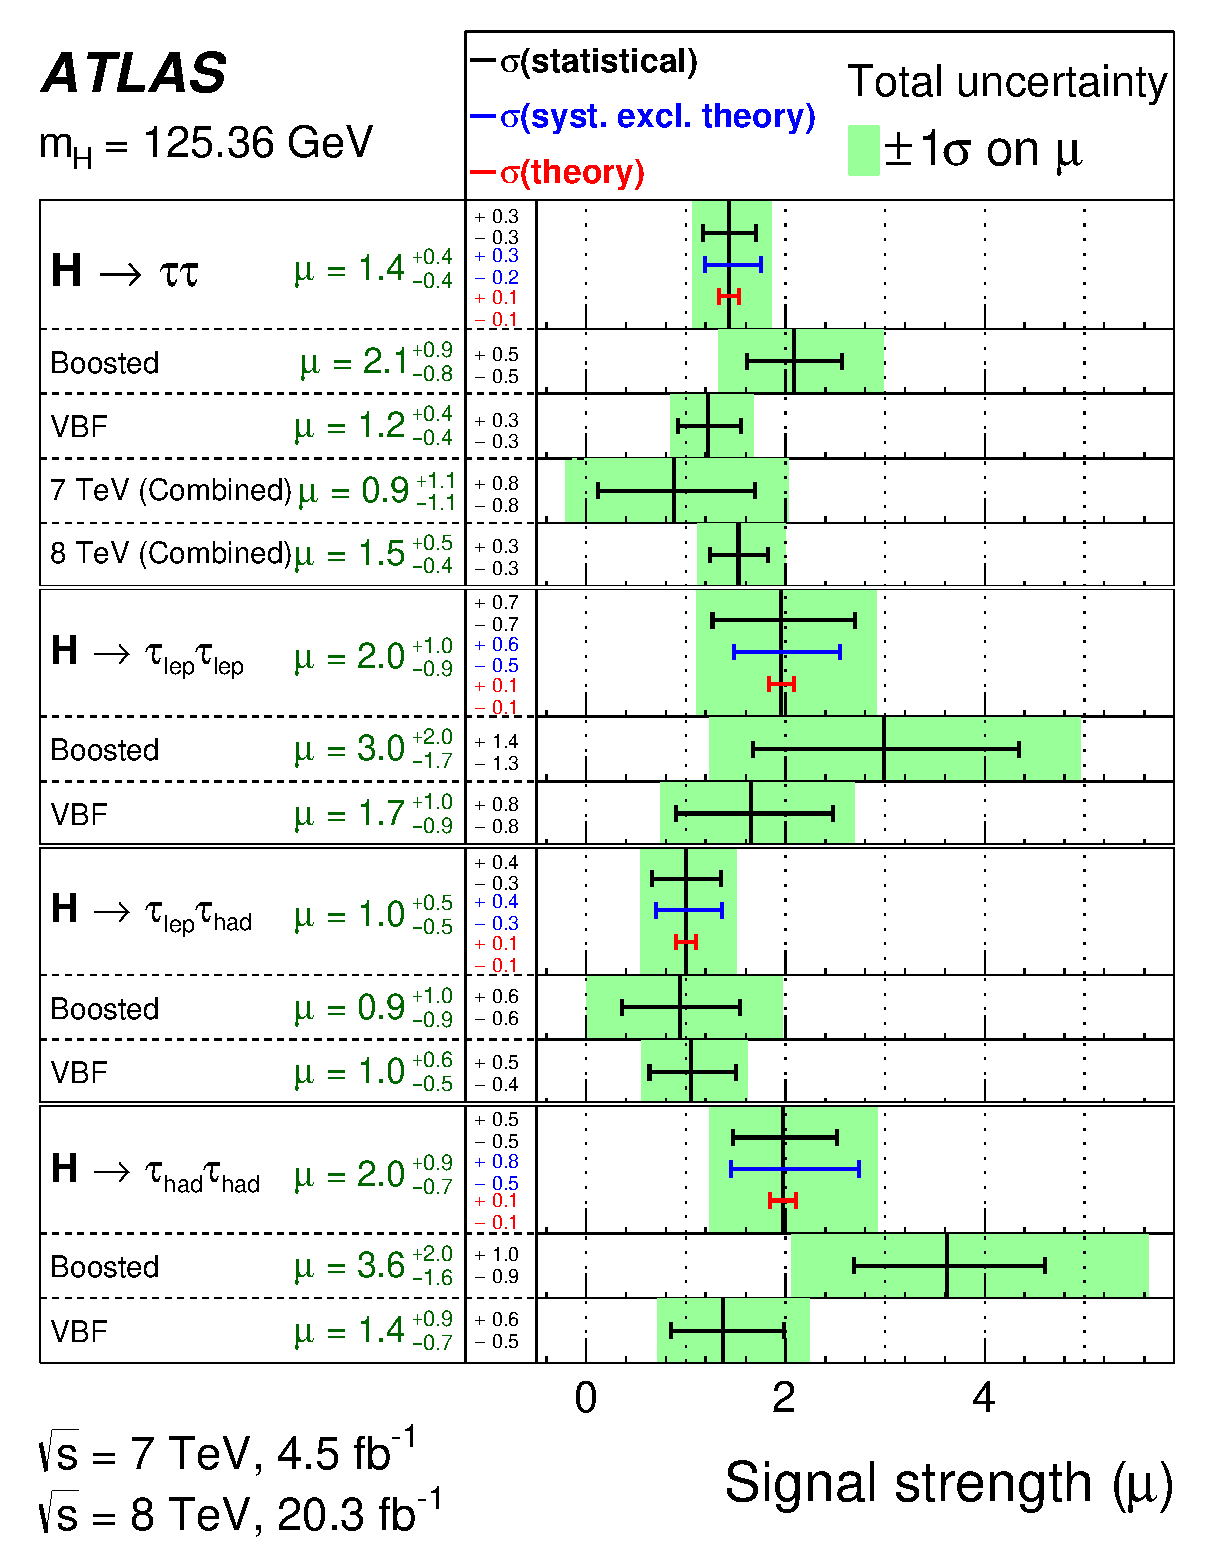
\includegraphics[width=0.90\textwidth]{figures/HIGG-2013-32/fig_09}
  \caption{The fitted signal strength $\mu$ split by category, final state, and data-taking period~\cite{HIGG-2013-32}.}
  \label{fig:results-musummary}
\end{figure}


